\chapter{Realizability of Polygonal Linkages with Fixed Orientation\label{chapter:polygonalLinkage}} 

We begin the chapter with describing several gadgets that translate the associated graph $A(\Phi)$ of a P3SAT boolean formula into a hexagonal polygonal linkage.  
These gadgets will be used together to form a special hexagonal linkage that behaves in a similar nature to the logic engine that encoded a NAE3SAT instance of Chapter \ref{chapter:logicEngine} but instead encodes a Planar 3-SAT and its associated graph.  
Given an instance $\Phi$ of P3SAT with $n$ variables and $m$ clauses and its associated graph $A(\Phi)$, 
Together the gadgets will form what is called the auxilary construction.
A hexagonal polygonal linkage and several gadgets enclosed in a frame (a frame that is conceptually similar to the frame found in a logic engine) would then be used to prove Theorem \ref{thm:hinge2}: \textit{it is strongly NP-hard to decide whether a polygonal linkage whose hinge graph is a \textbf{tree} can be realized with fixed orientation.}

Our proof is a reduction from P3SAT.
Given an instance $\Phi$ of P3SAT with $n$ variables and $m$ clauses and its associated graph $A(\Phi)$, we construct a simply connected polygonal linkage $(\PP,H)$ of polynomial size in $n$ and $m$, such that $\Phi$ is satisfiable if and only if $(\PP,H)$ admits a realization with fixed orientation. 


We construct a polygonal linkage in two main steps: first, we construct an auxiliary structure where some of the polygons have fixed position in the plane (called \emph{obstacles}), while other polygons are flexible, and each flexible polygon is hinged to an obstacle. 
Second, we modify the auxiliary construction into a polygonal linkage by allowing the obstacles to move freely, and by adding new polygons and hinges as well as an exterior \emph{frame} that holds the obstacle polygons in place.
All polygons in our constructions are regular hexagons or long, skinny rhombi.
In Chapter \ref{chp:disk} we can ``simulate'' these shapes with disk arrangements to show related results.

% In this paper we study the problem of orthogonal drawings,i.e., the drawing of a graph G = (V, E) where vertices are drawn as points and each edge is represented by a sequence of alternating horizontal and vertical segments. Such a representation is possible only when every vertex has at most four incident edges. Unless otherwise specified, we assume from now on that all graphs satisfy this condition. Then any graph G has an orthogonal drawing. In [11,16] it was shown that deciding whether G can be embedded in a grid of prescribed area is NP-complete. Sch~iffter showed that any graph can be embedded in a 2n x 2n-grid with at most two bends per edge [22]. For graphs with maximum degree 3, a very recent paper showed that they can be embedded in an rn/2~ x In/2] -grid with In/21 +2 bends [3]. If G is planar, it can be embedded in an n x n grid with 2n + 4 bends if it is biconnected, and 2.4n + 2 bends otherwise [23,25]. The number of bends along each edge is at most 4.
Storer, Tamassia, and Tollis \cite{storer1984minimal,tamassia1987efficient} showed that if $G=(V,E)$ is planar where $\vlr{V}=n$ and $\vlr{E} = m$, it can be embedded into a $\vert V \vert \times \vert V \vert$ integer grid where vertices are grid points and an edge are a sequence of alternating horizontal and vertical line segments and bounding total number of bends in an embedding by a bend polynomial $S(n,m)=2.4 \vert V\vert + 4$.  
Now suppose we're given a 3-CNF boolean formula, $\Phi$, with $i$ variables and $j$ clauses, the associated graph $A(\Phi)$ has $i+j$ vertices.  
We can then define a \textit{fundamental polynomial} $s(n,m)$ that describes the size of the embedding into the plane, $s(n,m) \times s(n,m)$, gives an upper bound on the total number of bends, and accounts for the translation of the associated graph of a P3SAT into a hexagonal polyonal linkage:
$$s(n,m) = 6\lr{3 (n+m) + 4} = 18 (n+m) + 24$$
Note that a planar bipartite graph has at most $2k-4$ by Euler's theorem where $k>2$.  
The tables below are a glossary of formulas and Maclaurin series that are used throughout this chapter.
It will serve as a useful reference for the reader.

$$
\begin{array}{|rcl|}
\hline
z(n,m)		&=& 4 s(n,m)\\\hline
J_h (n,m) 	&=& 6z(n,m)+1 = 24s(n,m)+1 \\\hline
J_d (n,m) 	&=& 4z(n,m)+1												= 16s(n,m)+1  			\\\hline
N(n,m)		&=& \frac{5t-1}{2}											= \frac{5s^\kappa-1}{2}	\\\hline
t(n,m)		&=& s^\kappa																		\\\hline
H(n,m) 		&=&  (12s+1)  \lr{5s^\kappa -1}  \sqrt{3} + 12s \lr{\sqrt{3}+ \frac{1}{250s^\kappa -50}}				\\\hline
\end{array}
$$


$$
\begin{array}{|rcl|}
\hline
&& x 				\leq \sin^{-1} x \leq x + \frac{x^3}{6} \qquad\qquad 0< x <1 \\\hline
&& x - \frac{x^3}{3}\leq \tan^{-1} x \leq x 				\qquad\qquad 0< x < 1\\\hline
&& \frac{x}{2}\leq x - \frac{x^3}{6}\leq \sin x 	 \leq x 				\qquad\qquad 0< x < 1\\\hline
&& 1 - \frac{x^2}{2}\leq \cos x 	 \leq 1 				\qquad\qquad 0< x < 1\\\hline
&& 1 				\leq \sec x 	 \leq 1 + \frac{x^2}{2} \qquad\qquad 0< x < 1\\\hline
\end{array}
$$
The formula $t(n,m)=s^\kappa$ has an exponent $\kappa$ which is a sufficiently large integer chosen later on so that all conditions in this chapter are satisfied.
The trigonmetric functions in the table above each are expressed as either the first term or the first and second term of their Maclaurin Series expansion.

\paragraph{Modifying the Associated Graph of a P3SAT.}

Given an instance of P3SAT boolean formula $\Phi$ of $n$ variables and $m$ clauses with associated graph $A(\Phi)$, we construct a finite \textit{honeycomb} grid $H_{A \lr{\Phi}}$ of regular hexagons over the plane.
We modify the associated graph $A\lr{\Phi}$ by embedding it into honeycomb integer grid in the following way:

\begin{enumerate}
%variables represent cycles of 2m 
\item \textbf{Variable:} A vertex representing a variable shall encompass a consecutive set of hexagons along a horizontal line in the honeycomb (see Figure \ref{fig:VariablesExample.pdf}).

\begin{minipage}{\linewidth}
\begin{center}
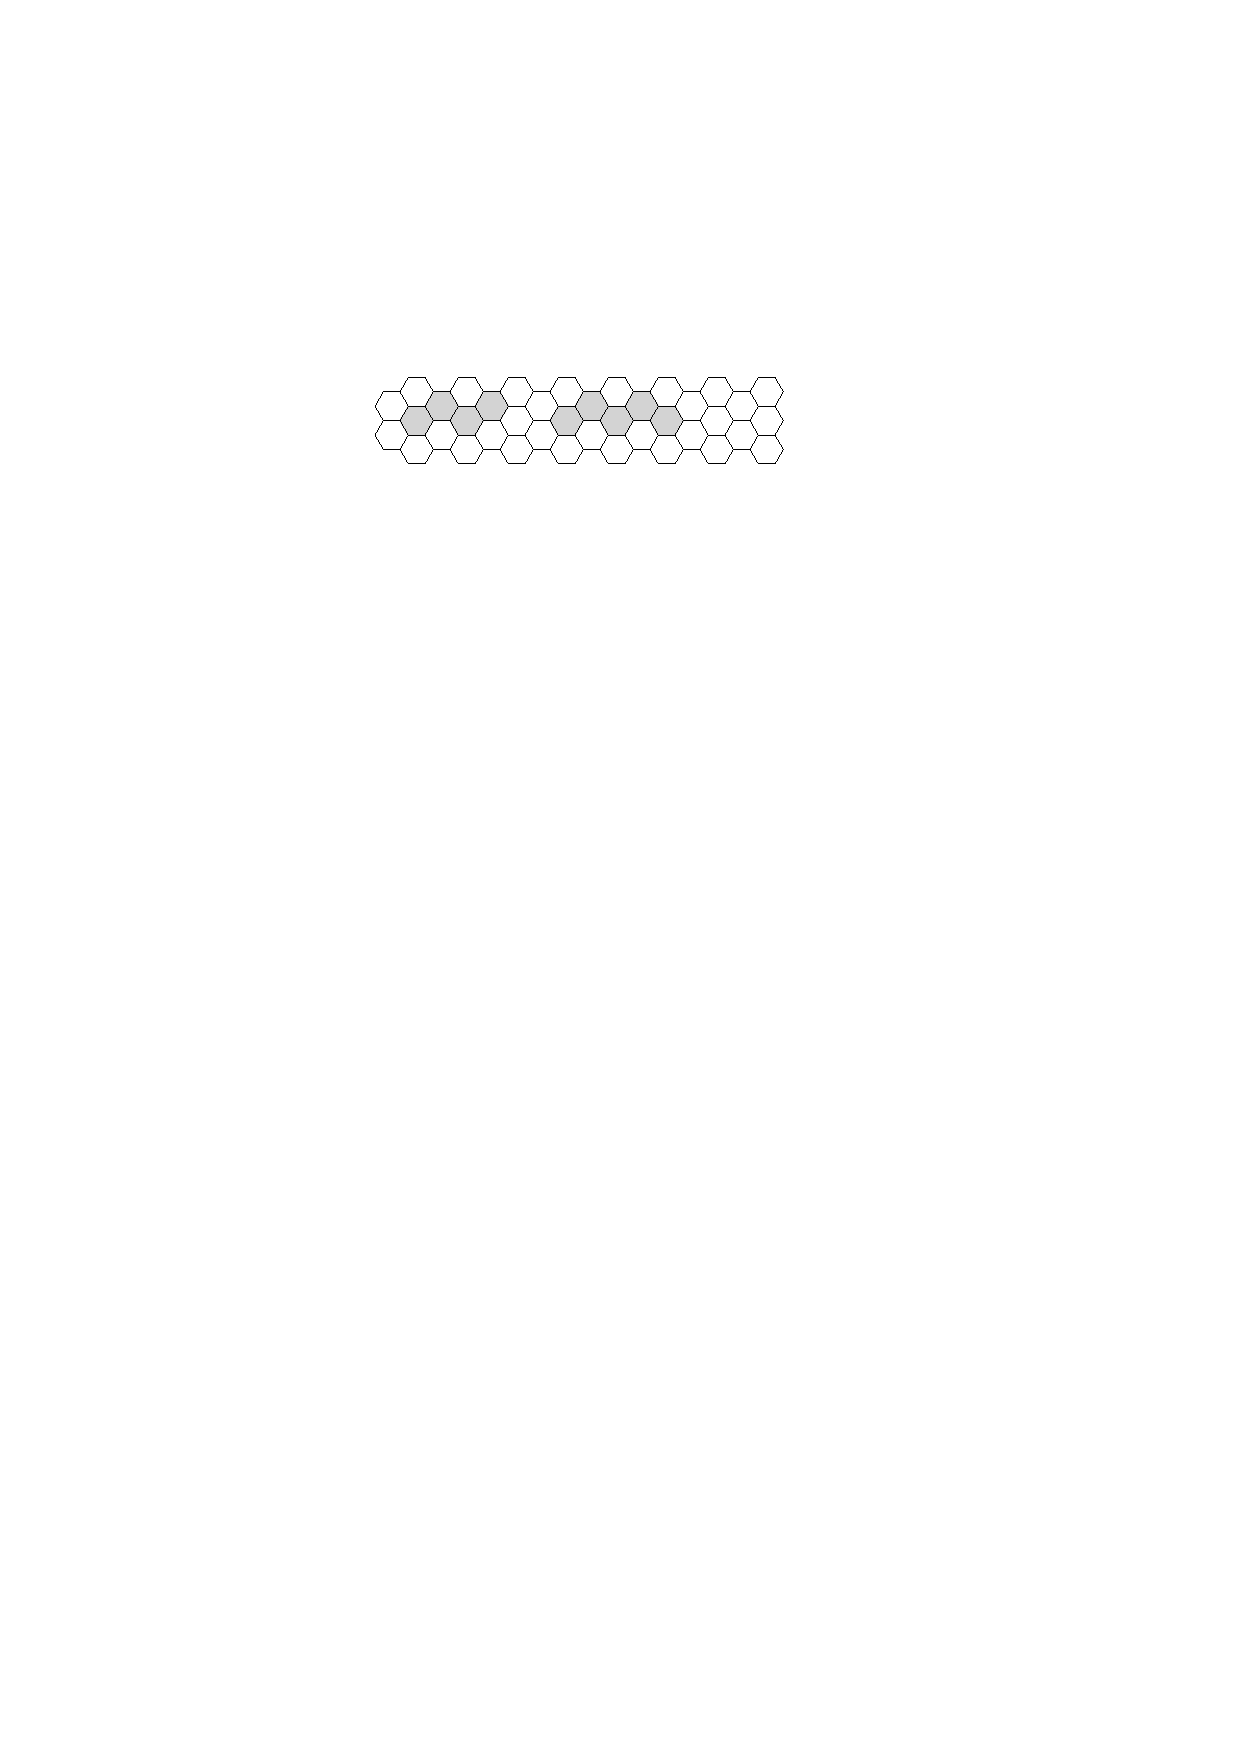
\includegraphics[width=.75\textwidth]{graphics/VariablesExample.pdf}
\captionof{figure}{The four shaded groups of horizontally adjacent hexagons represent four distinct variables from a boolean formula in the honeycomb.}\label{fig:VariablesExample.pdf}
\end{center}
\end{minipage}

Let $D = \max_{v \in V} \deg(v)$ where $V$ is the set of vertices of $A(\Phi)$.
Every variable vertex $v$  must encompass at least $2 \cdot \deg(v)$ consecutive hexagons but can encompass up to $2 \cdot D$ consecutive hexagons.
\item \textbf{Clause:} A vertex representing a clause shall be a vertex of a hexagon in the honeycomb.
\item \textbf{Edge:} Edges of the associated graph $A(\Phi)$ are paths between the variable $x_i$ and clause $C_j$.  An edge $\left\lbrace x_i, C_j \right\rbrace$ of the associated graph is pariwise edge disjoint. 
The edges of the drawing shall traverse the edges of hexagons in a vertically or horizontally zigzagging manner (see Figure \ref{fig:HoneyCombAssociatedGraphSmall}) in the honeycomb from the literal to the corresponding clause. 
Edges traverse a hexagon in two edges vertically, three edges horizontally.  
The vertical zigzagging edge segments traverse the left or right sides of a hexagon(s).
The horizontal zigzagging edge segments traverse the top or bottom halves of a hexagon(s).
When the edge transisitions from a vertical to horizontal traversal, the edge traverses in over 4 edges about the hexagon.
The length of the edges are bounded above by $6 \cdot \lr{\ell_1 \lr{x_i,C_j} + D}$ where $\ell_1$ is the $L_1$ norm and $x_i$ and $C_j$ are points in the grid plane. 
\end{enumerate}

\begin{minipage}{\linewidth}
\begin{center}
\includegraphics[width=.9\textwidth]{graphics/HoneyCombAssociatedGraphSideBySide.pdf}
\captionof{figure}{
(a) This is an instance of an associated graph for a P3SAT overlayed onto a honeycomb grid and placed into a regular hexagonal region.
This honeycomb graph could correspond to Boolean formula $\lr{\lnot x_1 \lor \lnot x_2 \lor x_4} \land \lr{x_2 \lor \lnot x_3 \lor x_4} \land \lr{x_1 \lor \lnot x_3 \lor \lnot x_4}$. (b) This is the same instance as (a) shown without the hexagonal region.
}\label{fig:HoneyCombAssociatedGraphSmall}
\end{center}
\end{minipage}

Figure \ref{fig:HoneyCombAssociatedGraphSmall} illustrates an associated graph of a P3SAT overlayed on a honeycomb.
Let the region in which the construction lies in be a regular hexagon region with polynomial side length $s(n,m)$. 
The honeycomb construction will act as preliminary concept that will be refined further in the Auxilary Contruction.
\section{Auxilary Construction}\label{sec:auxiliaryConstruction}
Let $\Phi$ be a Boolean formula of P3SAT with variables $x_1,\ldots , x_n$ and clauses $C_1,\ldots ,C_m$, where $A(\Phi)$ is the associated planar graph and $\tilde{A}\lr{\Phi}$ be corresponding honeycomb graph.
We continue to modify $\tilde{A}\lr{\Phi}$ to form the auxilary construction.   
Consider a large (polynomial-size) regular hexagon $J$  with side length $s(n,m)$ that contains all gadgets in our construction and hexagonal grid.
For each hexagon of the hexagonal grid contained in $J$, scale the hexagon in the following way: first we fix the center of the hexagon and then scale (shrink) the hexagon; adjacent hexagons in the honeycomb no longer touch each other and form corridors and junctions between the hexagons (See Figure \ref{fig:ScalingForCorridors.pdf}). 

\begin{minipage}{\linewidth}
\begin{center}
\includegraphics[width=.4\columnwidth]{graphics/ScalingForCorridors.pdf}
\captionof{figure}{(a) This figure shows a region of a hexagonal grid scaled in place to form corridors between adjacent hexagons(shown in (b)).}\label{fig:ScalingForCorridors.pdf}
\end{center}
\end{minipage}

Formally, let a \textit{corridor} be a channel between two adjacent hexagons and a \textit{junction} be a region where three corridors meet.

\textbf{Formal Decscription of the Auxilary Construction.}
Given the side length of $J$, $s(n,m)$, we need to scale the grid of hexagons of the hexagonal grid in the interior of $J$ accordingly.

\begin{minipage}{\linewidth}
\begin{center}
\includegraphics[width=.9\columnwidth]{graphics/hexagonalConstructionOfJSmallWithoutHalfHexagons.pdf}
\captionof{figure}{(a) shows a \textit{formal auxilary construction} with $k=2$. $k$ is the number of hexagons of the hexagonal grid in the interior of $J$ that is on the bottom most row.  (b) shows a formal auxilary construction with $k=3$. (c) shows a formal auxilary construction with $k=4$.  Note that in each figure}\label{fig:hexagonalConstructionOfJSmallWithoutHalfHexagons.pdf}
\end{center}
\end{minipage}

In Figure \ref{fig:hexagonalConstructionOfJSmallWithoutHalfHexagons.pdf}, we show the three smallest possible formal constructions of $J$, $J_1, J_2, J_3$.  
A formal construction of $J$ is when six hexagons of the hexagonal grid each have two adjacent sides lie on the perimeter of $J$.
We have shown informal construction earlier where this does not occur.
Unless otherwise specified, we will assume the use formal constructions.
Each of the figures in Figure \ref{fig:hexagonalConstructionOfJSmallWithoutHalfHexagons.pdf} shows $J$ in bold and the hexagonal grid in its interior.
Notice that in each case we have six hexagons of the hexagonal grid with each of the six hexgaons having two adjacent sides that lie on the perimeter of $J$.

The height and diamater of $J$ can be described in terms of hexagons in the grid a vertical or horizontal line may cross. 
We'll denote these qualities as the hexagonal height and hexagonal diameter of $J$.  
Figures \ref{fig:hexagonalConstructionOfJSmallWithoutHalfHexagons.pdf}(c) and \ref{fig:hexagonalConstructionOfJSmallWithoutHalfHexagons.pdf}(a) show the hexagons of the hexagonal height and hexagonal diamters of $J_1$ and $J_3$ respectively.  
The formula for calculating hexagonal height of $J_z$ is 
\begin{equation}\label{eqn:Jh}
J_h (n,m) = 6z(n,m)+1
\end{equation}
The formula for calcuating the hexagonal diameter of $J_z$ is 
\begin{equation}\label{eqn:Jd}
J_d (n,m) = 4z(n,m)+1
\end{equation}
Since the associated graph of a P3SAT instance can be encoded into a honeycomb grid of size $s(n,m) \times s(n,m)$, then let $z(n,m)=4\cdot s(n,m)$ to enclose the same honeycomb to be enclosed into the interior of $J_z$.

% Figure \ref{fig:hexagonalConstructionOfJSmallWithoutHalfHexagons.pdf}(b) illustrates the side length of $J$ as $s(n,m)$ and half the height of $J$ as $s(n,m) \sqrt{3}$.
% For any $J$, there is a fixed number of hexagons in the hexagonal grid that lie on one side of the perimeter of $J$; denote this number as $k$.
% We can denote the number of hexagons in a row of the hexagonal grid in $J_z$ with the following sequence as follows:
% \begin{equation}\label{eqn:hexagonalGridSequence}
% \begin{array}{rcl}
% a(0) &=& k\\
% a(1) &=& k-1 \\
% a(2) &=& k\\
% a(i) &=& a(i-3)+1\\
% 0\leq&i&\leq \ceil{\frac{J_h (z)}{2}}
% \end{array}
% \end{equation}
% The $i^\text{th}$ number of Sequence \ref{eqn:hexagonalGridSequence} indicates the number of hexagons on the $i^\text{th}$ row of the hexagonal grid in the interior of $J$ from the perimeter of $J$ up to the half height of $J$. In Figure \ref{fig:hexagonalConstructionOfJSmallWithoutHalfHexagons.pdf}(c) from the bottom to the mid-height of $J$, the sequence $a(i)$ (i.e. the number of hexagons in each subsequent row) is 4, 3, 4, 5, 4, 5, 6, 5, 6, 7.
% Denote the hexagons of the hexagonal grid in $J$ as \textit{obstacle hexagons}.

\begin{minipage}{\linewidth}
\begin{center}
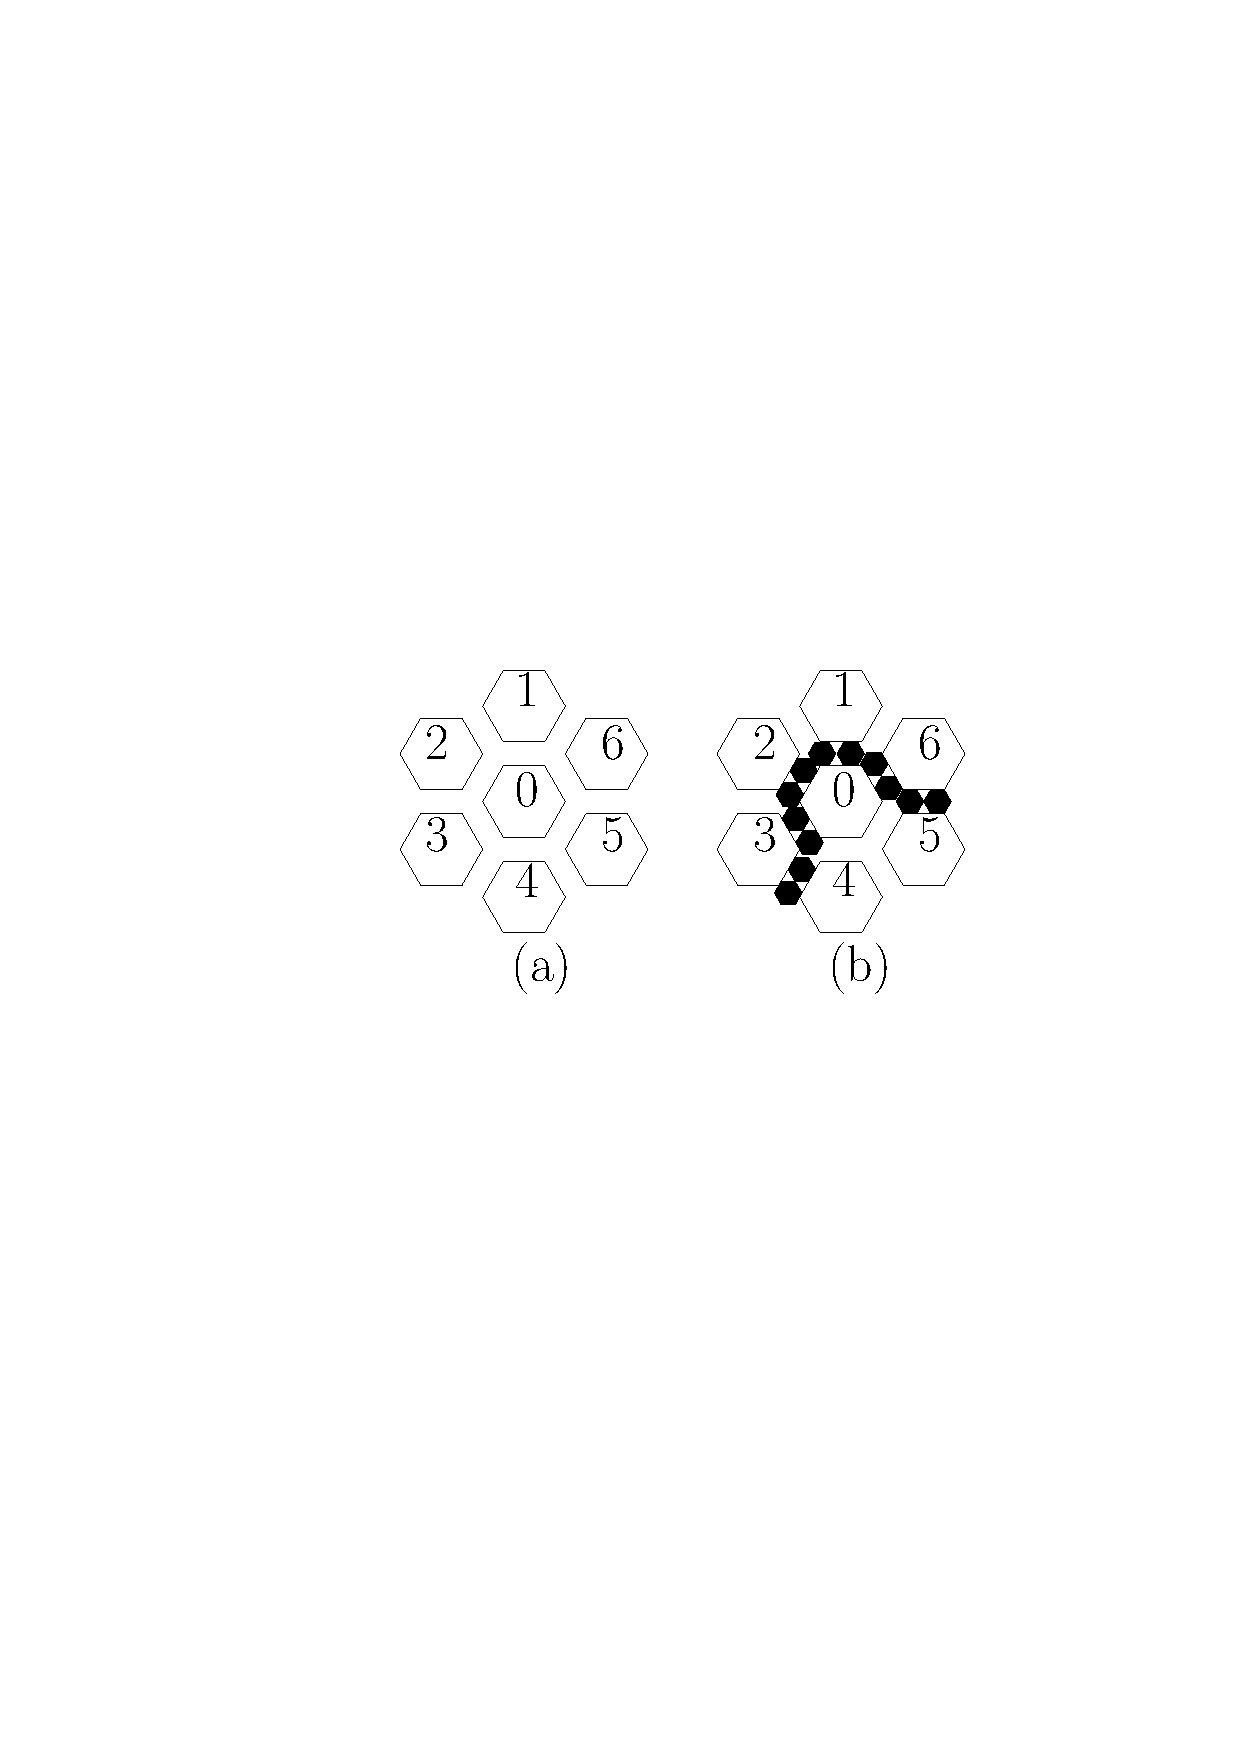
\includegraphics[scale=.66]{graphics/FlexibleHexagons.pdf}
\captionof{figure}{
(a) A region of the honeycomb shown with scaling. The corridors and junctions formed from the first scaling is preserved after scaling the honeycomb grid to where the side lengths of the hexagon are $N(n,m)$.
(b) The same region in (a) containing flags.
}\label{fig:HoneycombFlixible.pdf}
\end{center}
\end{minipage}



The obstacle hex Figure \ref{fig:HoneycombFlixible.pdf}(a) be obstacle hexagons that are fixed.
In Figure \ref{fig:HoneycombFlixible.pdf}(b), we have smaller hexagons within some corridors and junctions.
These hexagons are flags.
For each edge in $\tilde{A}(\Phi)$, we insert flags into the corridor corresponding to that edge.
%Flags are hinged at the vertex closest to origin and the side of the corridor (See Figure \ref{fig:variable}).
Flags are regular hexagons that reside in the corridors and junctions; each flag is hinged to a obstacle hexagon (see Figure \ref{fig:HoneycombFlixible.pdf}(b)).  
For any of these corridors, we attach hinges to the boundary of the corridor; pick an arbitrary side for all hinges.  
The first and last hinge are one unit from the obstacle hexagon corners, the hinges between the first and last hinge are 2.5 units apart.  
Let $t(n,m)=s^\kappa$ be the number of flags in a corridor (see Figure \ref{fig:variable}). 
Scale $J$ and the obstacle hexagons in the interior of $J$ independently from their centers (see Figure \ref{fig:ScalingForCorridors.pdf}) such that each obstacle hexagon has side length: $$N(n,m)=\frac{5t(n,m)-1}{2}.$$ 

\begin{minipage}{\linewidth}
\begin{center}
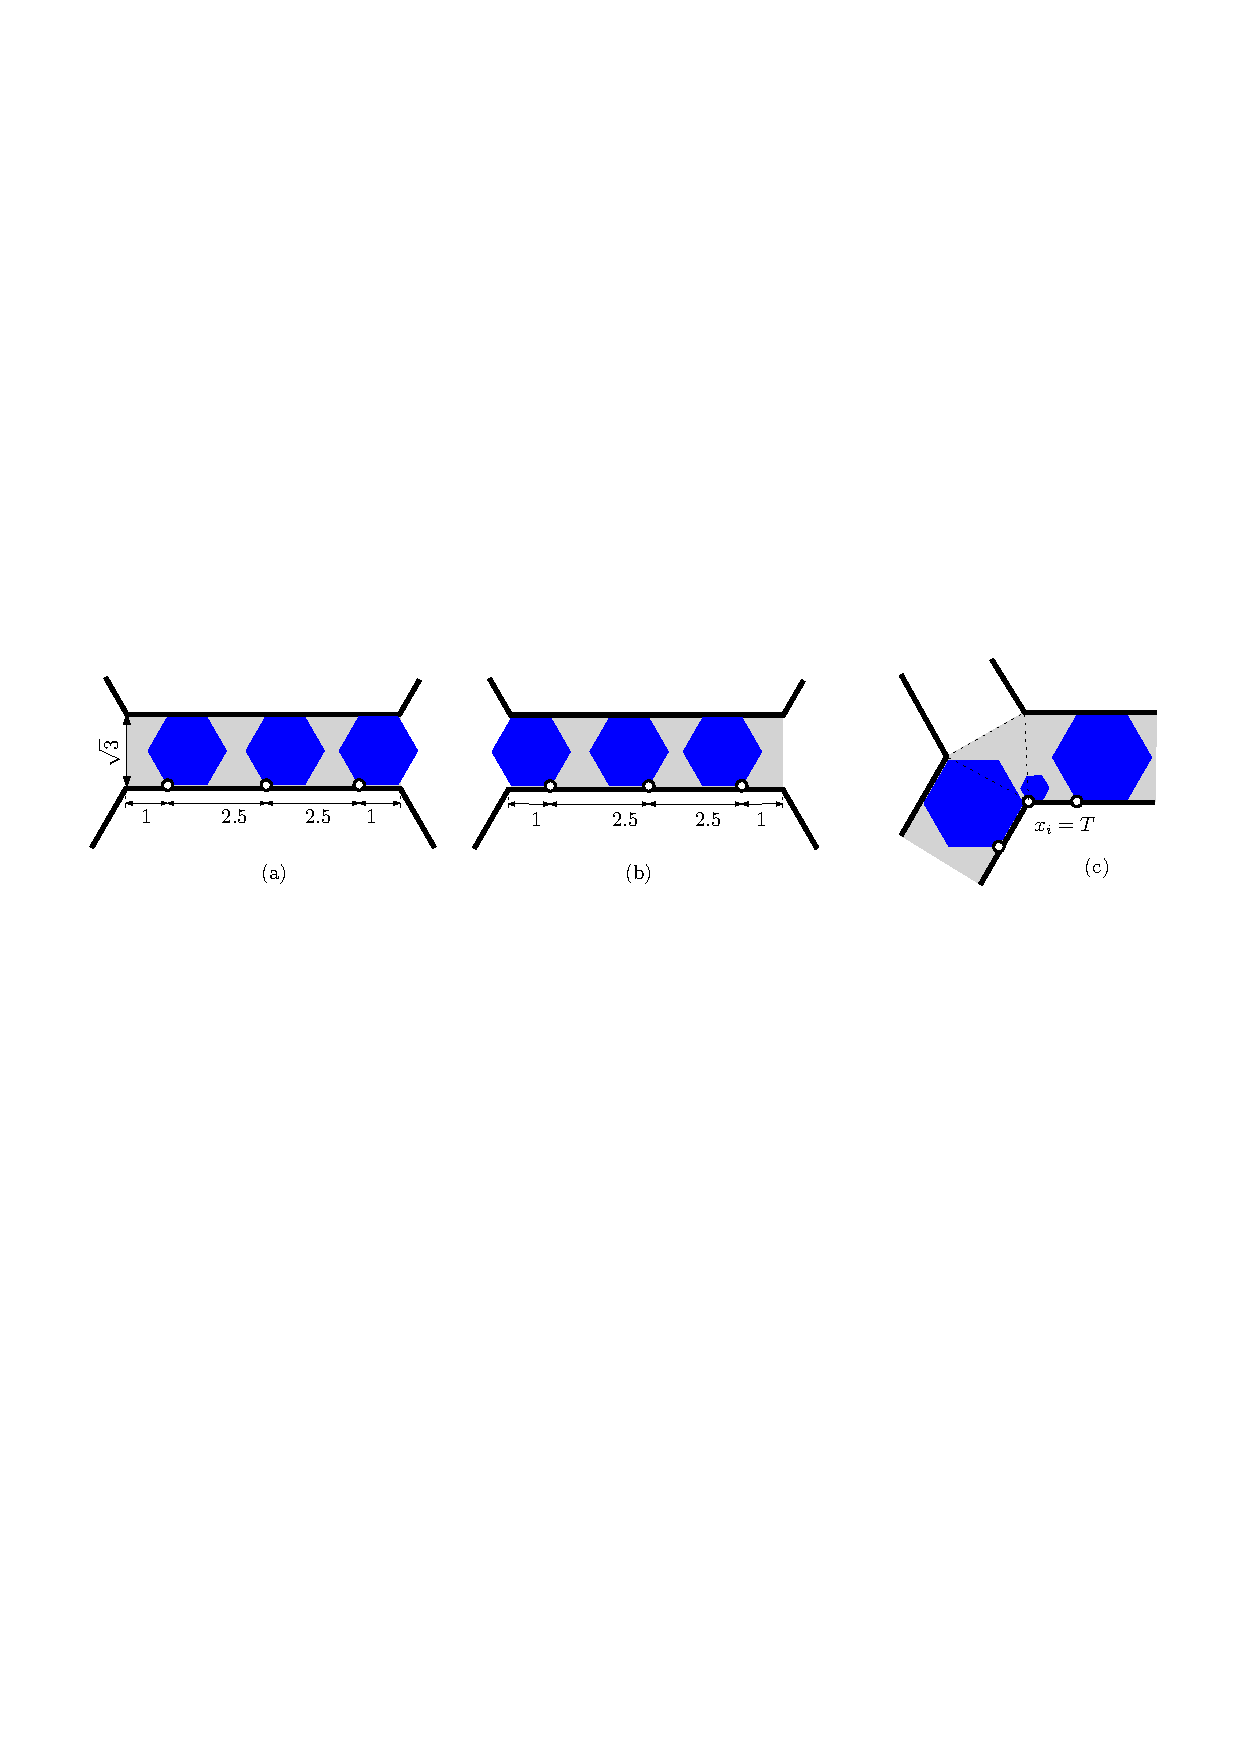
\includegraphics[width=0.9\columnwidth]{graphics/fig-variable-hex+}
\captionof{figure}{
(a) A corridor when all unit hexagons are in state R.
(b) A corridor where all unit hexagons are in state L.
(c) A junction where a small hexagon between two corridors
    ensures that at most one unit hexagon enters the junction from those corridors.}\label{fig:variable}
\end{center}
%\end{figure}
\end{minipage}

%These large hexagons are considered fixed obstacles in our auxiliary construction. 
Between two adjacent obstacle hexagons, there is a $\frac{5t-1}{2}\times \sqrt{3}$ rectanglar corridor.  %, which we call corridor. 
Three adjacent corridors meet at a regular triangle, which we call a junction. 

We next describe variable, clause, and transmitter gadgets.
The basic building block of both variable and transmitter gadgets consists of $t$ regular hexagons of side length 1 (\emph{unit hexagons}, for short) attached to a wall of a corridor such that the hinges divide the wall into $t+1$ intervals of length $(1,2.5,\ldots ,2.5,1)$ as shown in Fig.~\ref{fig:variable}(a-b). 

% In some of the junctions, we attach a small hexagon of side length $\frac{1}{3}$ to one or two corners of the junction (see Fig.~\ref{fig:variable}(c) and Fig.~\ref{fig:transmitter}). 

\paragraph{Variable Gadget.}
The {\bf variable gadget} for variable $x_i$ is constructed as follows. 
Recall that variable $x_i$ corresponds to a cycle in the associated graph $\tilde{A}(\Phi)$, which has been embedded as a cycle in the hexagonal tiling, with corridors and junctions. 
In each junction along this cycle, attach a small hexagon in the common boundary of the two corridors in the cycle. 
Figure \ref{fig:VariableGadgetSmall.pdf} depicts a \textit{variable gadget} in the hexagonal grid.

\begin{minipage}{\linewidth}
\begin{center}
\includegraphics[width=0.45\columnwidth]{graphics/VariableGadgetSmall.pdf}
\captionof{figure}{This depicts a variable gadget with $x_1 = T$.  Carefully note that the flags around $x_1$ are in the state $R$. Corridors adjacent to two obstacles of a variable in the honeycomb do not have $t$ flags; these corridors simply have the flags at the junctions.}\label{fig:VariableGadgetSmall.pdf}
\end{center}
\end{minipage}

For each junction in the transmitter gadget, we attach a small hexagon in the junction as shown in Figure \ref{fig:transmitter} except at the clause junction.
 A {\bf transmitter gadget} is constructed for each edge $\left\lbrace x_i,C_j\right\rbrace$ of the graph $A(\Phi)$; it consists of a sequence of junctions and corridors from a variable gadget's junction to a clause junction.  
Choosing the location of the small hexagon depends on whether the non-negated or negated literal is found in the clause.
\begin{itemize}
\item[(a)]  For an edge $(x_i,C_j)$ of the graph $A(\Phi)$, if the non-negated literal of $x_i$ exists in $C_j$, attach the small hexagon to the left side of the junction (see Figure \ref{fig:VariableJunctionTransmitterSelection.pdf}(a)).
\item[(b)]  For an edge $(x_i,C_j)$ of the graph $A(\Phi)$, if the negated literal of $x_i$ exists in $C_j$, attach thhe small hexagon to the right side of the junction (see Figure \ref{fig:VariableJunctionTransmitterSelection.pdf}(b)).
\end{itemize}
\paragraph{Clause Gadget.}
Recall that a clause from a Boolean formula $\Phi$ in 3-CNF has three literals.  If $\Phi$ is a  'yes' instance, then at least one literal in every clause of $\Phi$ is true.  We construct the clause gadget to model this fact about Boolean formulas in 3-CNF.

The {\bf clause gadget} lies at a junction adjacent to three transmitter gadgets (see Fig.~\ref{fig:clause} and Section \ref{transmitterGadget}). 
At such a junction, we attach a unit line segment to an arbitrary vertex of the junction, and a small hexagon of side length $\frac{1}{3}$ to the other end of the segment. 
If unit hexagons enter the junction from all three corridors (i.e., all three literals are false), then there is no space left for the small hexagon (see Lemma \ref{lem:aux-1}).

\begin{minipage}{\linewidth}
\begin{center}
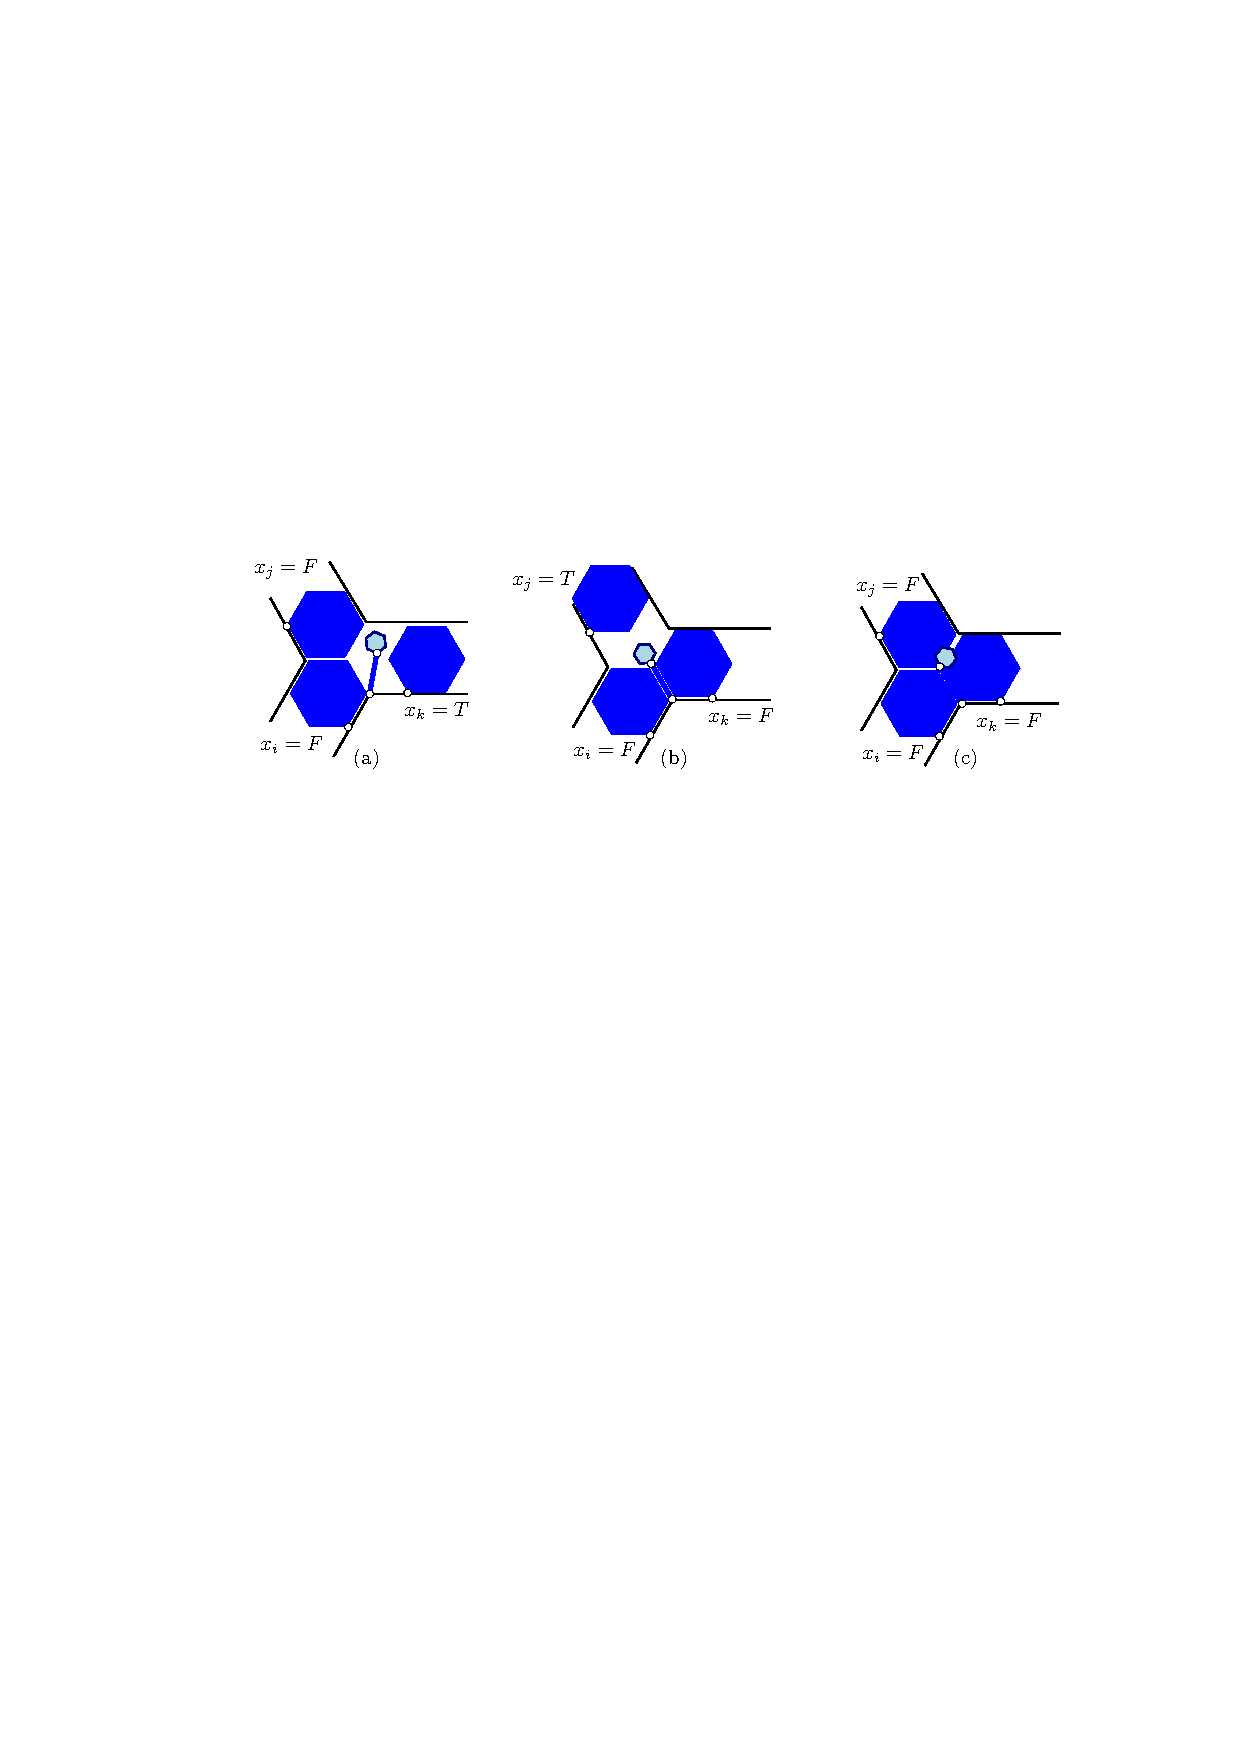
\includegraphics[width=0.7\columnwidth]{graphics/fig-clause-hex}
\captionof{figure}{(a-b) A clause gadget $(x_i\vee x_j\vee x_k)$ i\
    realizable when at least one of the literals is {\sc True}.
    (c) The clause gadget cannot be realized when all three literals are {\sc False}.}\label{fig:clause}
\end{center}
\end{minipage}

%But if at most two unit hexagons enter the junction (i.e., one of the literals is true), then the unit segment and the small hexagon are realizable.

\paragraph{Transmitter Gadget.\newline }\label{transmitterGadget}

\begin{minipage}{\linewidth}
\begin{center}
\includegraphics[width=0.7\columnwidth]{graphics/fig-assoc-hex}
\captionof{figure}{Left: the associated graph $A(\Phi)$ for a Boolean formula $\Phi$.
Right: the schematic layout of the variable, clause, and transmitter gadgets in the auxiliary construction showing in Section \ref{sec:auxiliaryConstruction}}\label{fig:assoc2}
\end{center}
\end{minipage}

In the associated planar 3-SAT graph $A(\Phi)$, every variable vertex has an cyclic order of edges.
Suppose we have a variable vertex $x_i$ with counter-clockwise cyclic order of edges $\left(\left\lbrace x_i,C_1\right\rbrace\right.$, $\left\lbrace x_i,C_2\right\rbrace$, $\dots$, $\left.\left\lbrace x_i,C_k\right\rbrace\right) $.  
Assign distinct junctions of the variable cycle of $x_i$ to the edges $\left\lbrace x_i,C_j\right\rbrace$ in the same cyclic order (refer to Figure \ref{fig:assoc2} for an example).

\begin{minipage}{\linewidth}
\begin{center}
\includegraphics[width=0.80\columnwidth]{graphics/VariableJunctionTransmitterSelection2.pdf}
\captionof{figure}{These two figures depict an example of placing a transmitter gadget corresponding to edge $\left\lbrace x_i, C_j \right\rbrace$.}
\label{fig:VariableJunctionTransmitterSelection.pdf}
\end{center}
\end{minipage} 

Figure \ref{fig:VariableJunctionTransmitterSelection.pdf} shows an example of each rule on choosing a junction to attach a transmitter gadget.
% The first column transmits a ``true'' value between the variable gadget and clause junction.
% The second column transmits a ``false'' value between the variable gadget and clause junction.
In this figure, both variable gadgets are in state $R$, i.e. variable $x_i = T$.  
Figure \ref{fig:VariableJunctionTransmitterSelection.pdf}(a) we have a transmittion of ``true'' between the variable and clause gadget.
% The variable gadgets in the second row are are in state $L$, i.e. variable $x_i = F$.

\begin{minipage}{\linewidth}
\begin{center}
	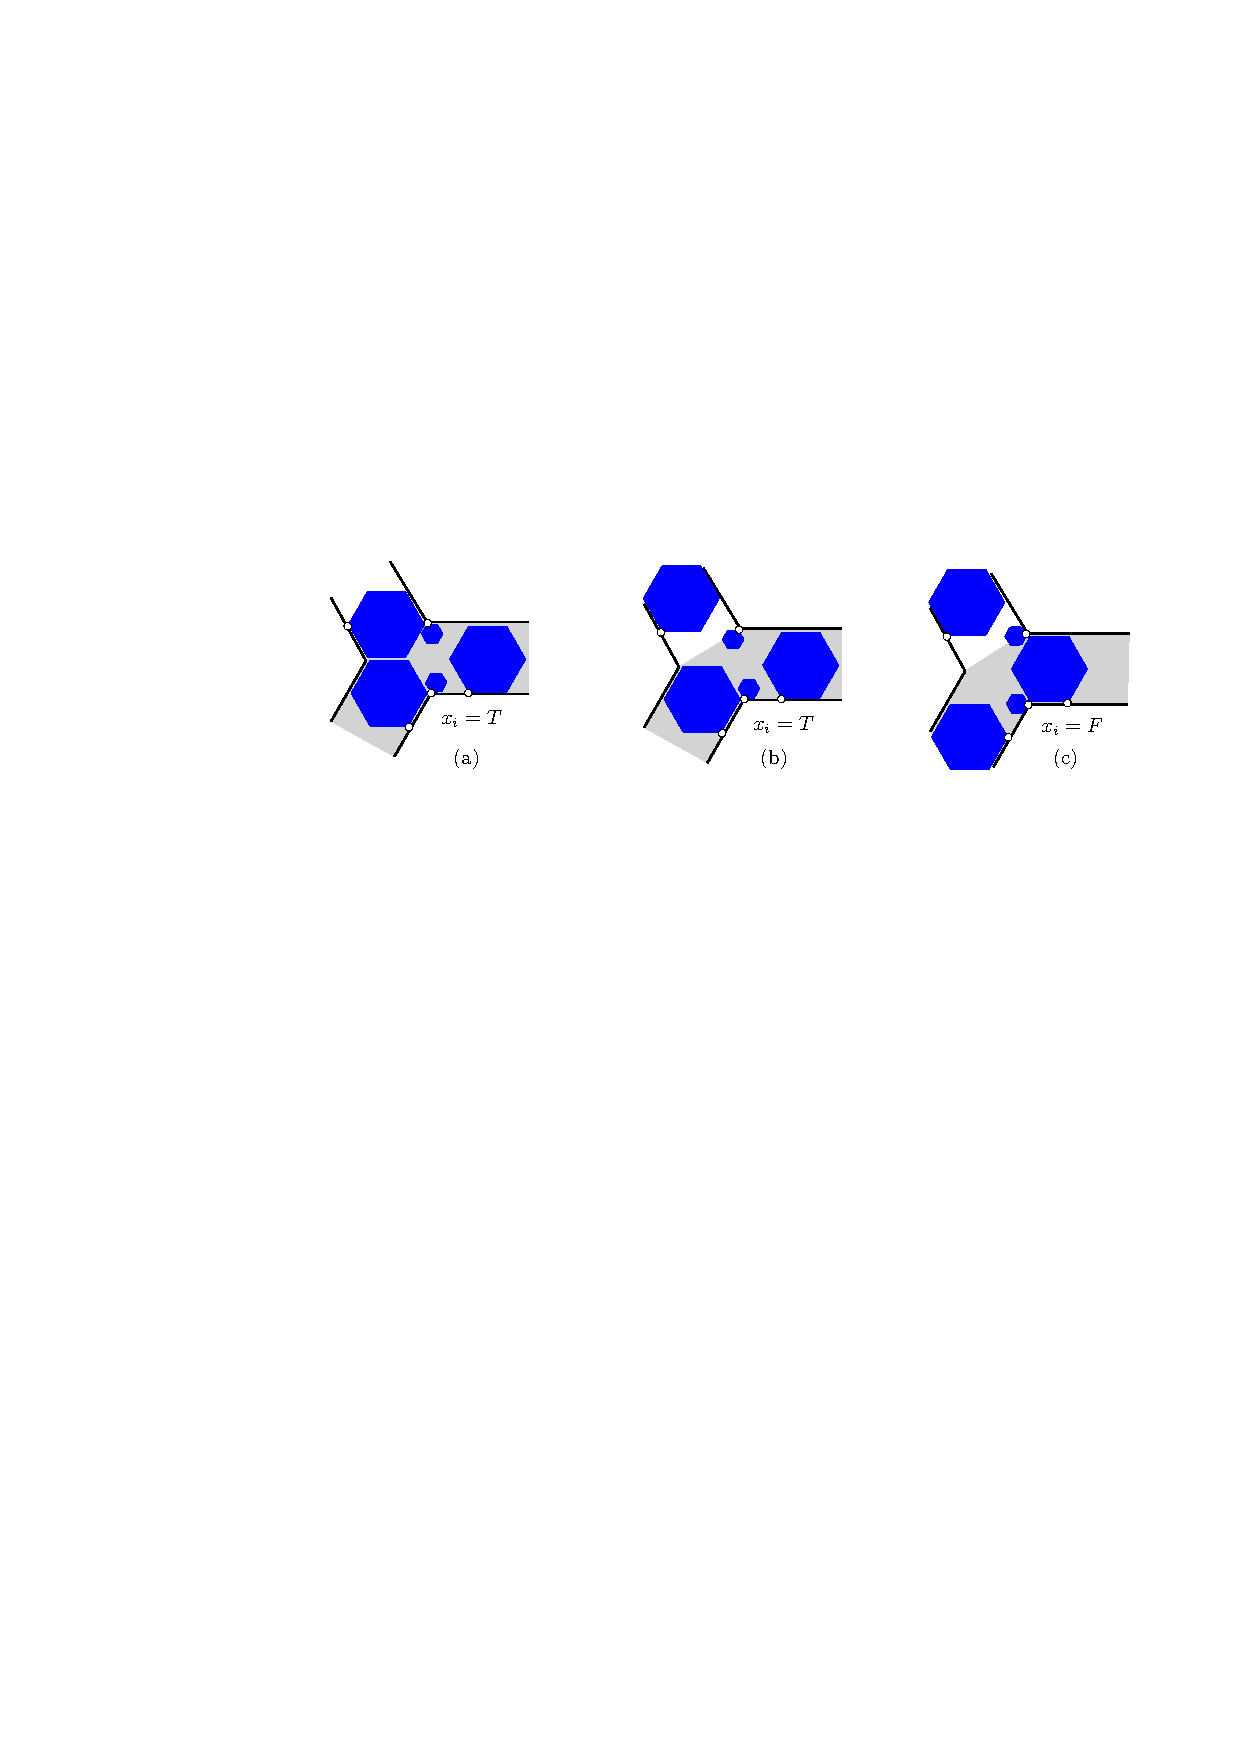
\includegraphics[width=0.7\columnwidth]{graphics/fig-transmitter-hex}
	\captionof{figure}{The common junction of a variable gadget and a transmitter gadget.
(a) When $x_i=T$, a hexagon of the transmitter may enter the junction of the variable gadget.
(b) When $x_i=T$, the transmitter gadget has several possible realizations.
(c) When $x_i=F$, no hexagon from the transmitter enters a junction of the variable gadget.}
	\label{fig:transmitter}
\end{center}
\end{minipage} 

This completes the description of the auxiliary construction.

\section{Functionality of the Auxilary Construction and Gadgets}

For each corridor, there are two junctions adjacent to it; of these two junctions, we denote the junction from which a flag in the corridor enters into as the \textit{active junction} (see Figure \ref{fig:ActiveChannel.pdf}).  
% If the literal $x_i$ (resp., $\overline{x}_i$) appears in $C_j$, then we attach a small hexagon to the corner of this junction such that if $x_i=F$ (resp., $\overline{x}_i=F)$, then the unit hexagon of the transmitter gadget cannot enter this junction. 

\begin{minipage}{\linewidth}
\begin{center}
\includegraphics[width=0.9\columnwidth]{graphics/ActiveChannel.pdf}
\captionof{figure}{The active junction in (a) is the junction on the left and in (b) the active junction is on the right.  The active junction is the junction in which a flag enters from a corridor.}\label{fig:ActiveChannel.pdf}
\end{center}
\end{minipage}

% A variable gadget for vertex $v$ in the associated graph of a P3SAT Boolean formula encompasses at least $2 \cdot \deg (v)$ consecutive obstacle hexagons. 
% The arrangement of the consecutive obstacle hexagons are in staggered fashion about a horizontal line where there are at least $\deg (v)$ obstacle hexagons in the upper portion of the staggering arrangement and at least $\deg (v)$ obstacle hexagons in the lower portion of the staggering arrangement.

Section \ref{sec:auxiliaryConstruction} is a formal description of the auxilary construction and its gadgets.
This subsection covers the underlying assumptions and proofs about the functionality of the auxilary construction.
Throughout this section we assume that the polygonal linkage is realizable, i.e. no two polygons overlap.  
The first observations about the functionality of the auxilary construction are about the flags.  
For $t$ flags in a corridor, the following holds:
\begin{observation}\label{obs:corridor}
\begin{itemize}
\item[(1)] If the leftmost flag is in state R, then all $t$ flags are in state R, and the rightmost flag enters the junction on the right of the corridor.
\item[(2)] Similarly, if the rightmost flag is in state L, then all $t$ flags are in state L, and the leftmost flag enters the junction on the left of the corridor.
\end{itemize}
\end{observation}

Observation~\ref{obs:corridor} and the small hexagons ensure that the state of any flag along the cycle determines the state of all other unit hexagons in the cycle. 
This property defines the binary variable $x_i$: if all flags in the top horizontal corridors are in state R and $x_i=F$, then $x_i=T$ and all hexagons are all in state L.

When a binary variable $x_i = T$, we will say that the variable in state $R$ and that the cycle of small hexagons around the variable gadget are in a ``clockwise direction''.
When a binary variable $x_i = F$, we will say that the variable is in state $L$ and that the cycle of small hexagons around the variable gadget are in a ``counter-clockwise direction''. 

The proof of the Observation \ref{obs:corridor} is similar to the proof of Lemma \ref{lem:logicEngine1} regarding a row in a logic engine having a collision-free configuration.
\begin{proof}
Suppose the leftmost hexagon, $h_1$, is in state $R$ in a corridor.
Denote the $t$ flags in a corridor as $h_1$, $h_2$, $\ldots$, $h_t$ from leftmost to rightmost respectively.
$h_2$ must be in state $R$ otherwise we result in a collision between $h_1$ and $h_2$.
Without losss of generality, $h_i$ and $h_{i+1}$ must be in a state $R$ in order to prevent an adjacent flag collision. 
This implies that rightmost flag $h_t$ must also be in state $R$; this implies that $h_t$ enters the junction that is on the right of the corridor.

Similarly, suppose the rightmost hexagon, $h_t$, is in state $L$ in a corridor.
Denote the $t$ flags in a corridor as $h_1$, $h_2$, $\ldots$, $h_t$ from leftmost to rightmost respectively.
$h_{t-1}$ must be in state $L$ otherwise we result in a collision between $h_t$ and $h_{t-1}$.
Without losss of generality, $h_i$ and $h_{i+1}$ must be in a state $L$ in order to prevent an adjacent flag collision. 
This implies that rightmost flag $h_1$ must also be in state $L$; this implies that $h_1$ enters the junction that is on the left of the corridor.
\end{proof}

% Each junction is a regular triangle, adjacent to three corridors. 
% In some of the junctions, we attach a small hexagon of side length $\frac{1}{3}$ to one or two corners of the junction (see Fig.~\ref{fig:variable}(c) and Fig.~\ref{fig:transmitter}). 
% Importantly, we have the following observation:
\begin{observation}\label{obs:junction}
If a small hexagon is attached to a vertex at a junction between two adjacent corridors, then a flag can enter the junction from at most one of those corridors.
\end{observation}
\begin{proof}
Suppose there is a small hexagon attached to a vertex at a junction between two adjacent corridors.
Suppose it is not that case that a flag can enter the junction from at most one of these adjacent corridors.
Then there are two flags entering the junction, one from each adjacent corridor.
The angular sum of the vertex about the adjacent corridors consists of the obstacle hexagon, both flags, and the small unit hexagon.
Each angle of each hexagon is $\frac{2 \pi}{3}$ radians, totalling to an angular sum of $\frac{8 \pi}{3} > 2 \pi$.
This is a contradiction with the total angular sum of a vertex on the plane to be $2 \pi$.
\end{proof}

The flags of the auxilary construction help communicate the boolean value of a variable gadget to the rest of the auxilary construction.
This property of the flags in a corridor is analagous to the flags in a row of a logic engine.

Observations \ref{obs:corridor} and \ref{obs:junction} ensure that the state of any unit hexagon along the cycle determines the state of all other unit hexagons in the cycle. 
This property defines the binary variable $x_i$: If $x_i=T$, then all unit hexagons in the top horizontal corridors are in state R; and if $x_i=F$, they are all in state L.

For a variable gadget $x_i$, we distinguish the upper half and lower half of the gadget in the variable cycle.
Then we have the following lemma:
\begin{lem}\label{lem:aux-2}
If variable $x_i = T$, then all flags in the upper half of the variable gadget are in state $R$ and all flags in the lower half of the variable are in state $L$; if variable $x_i = L$, then all flags in the upper half of the variable gadget are in state $L$ and all flags in the lower half of the variable gadget are in state $R$.    
\end{lem}
This lemma servers to show that the truth or falsity of a variable is consistent throughout the gadget.
\begin{proof}
Suppose we have two adjacent corridors $k_i$ and $k_{i+1}$ sharing junction $J_i$ and without loss of generality, $k_i$ is the left most corridor.
Observation \ref{obs:junction} implies that there can only be one hexagon entering $J_i$ from either $k_i$ or $k_{i+1}$. If the hexagon that enters $J_i$ is from corridor $k_i$, then this hexagon has state $R$ and all flags in corridor $k_i$ are in state $R$ by Observation \ref{obs:corridor}. 
Since the nearest flag of corridor $k_{i+1}$ cannot enter the junction $J_i$, it must also have state $R$.  
All flags in corridor $k_{i+1}$ are in state $R$ by Observation \ref{obs:corridor}. 

The argument is similar if the hexagon entering $J_i$ is from corridor $k_{i+1}$ and all flags in both corridors $k_i$ and $k_{i+1}$ have state $L$.

Because variable gadgets form a simple cycle of corridors and junctions $\lr{k_1, J_1, k_2, J_2, \dots, k_n, J_n}$ and the argument above, all flags about a variable gadget have the same state.
\end{proof}

Suppose there is an edge $\left\lbrace x_i, C_j \right\rbrace$ in the graph $A(\Phi)$:
\begin{lem}\label{lem:aux-3}
If $x_i = T$ and its negated literal is in $C_j$, then a flag enters into the clause gadget of $C_j$, otherwise it need not enter; if $x_i = F$ and its non-negated literal is in $C_j$, then a flag enters into the clause gadget of $C_j$, otherwise it need not enter.
\end{lem}
\begin{proof}
The transmitter gadget for each literal is placed on an active junction of the variable gadget. 
This junction is ``activated'' by the variable gadget.  
By Observation \ref{obs:junction}, the flag nearest of the transmitter gadget to the variable gadget does not enter the transmitter-variable junction.
By Observation \ref{obs:corridor} and the state of the flag nearest of the transmitter gadget to the variable gadget implies that the flags in that transmitter corridor activate the junction opposite the transmitter-variable junction.
The subsequent flags in the transmitter gadget corridors have the same state of the flag in the transmitter gadget nearest of the transmitter-variable junction by Observations \ref{obs:corridor} and \ref{obs:junction}.
This activation process continues up to the clause junction and the flag in the transmitter gadget nearest the clause junction enters the clause junction.
\end{proof}

\begin{lem}\label{lem:aux-1}
Hexagons in a clause junction have a non-overlapping placement if and only if at least one of the three literals is true.
\end{lem}
\begin{proof}
Suppose we have a hexagons in a clause junction that have a non-overlapping placement.
To show that there is at least one of the three literals is true,  we do a proof by contradiction.
Suppose all literals of the clause are false.
If all literals of the clause are false, then all flags in each transmitter gadget nearest their clause junction enters the clause junction, as shown in Figure \ref{fig:clause}(c) which show the small hexagon overlapping flags in the clause junction, a contradiction with hexagons in the clause junction have a non-overlapping placement.

If at least one of the three literals is true, then by Lemma \ref{lem:aux-3}, this literal's flag need not enter the transmitter-variable junction.
There allows for the small hexagon in the clause junction to move into the area where this literal's flag could enter the junction and thus allow non-overlapping placement of hexagons in the junction.
\end{proof}



\begin{lem}\label{lem:aux-A}
For every instance $\Phi$ of P3SAT, the above polygonal linkage with flexible and obstacle polygons has the following properties: (1) it has polynomial size; (2) its hinge graph is a forest;
(3) it admits a realization such that the obstacle polygons remain fixed if and only if $\Phi$ is satisfiable.
\end{lem}
\begin{proof}

We can bound the number of obstacle hexagons to represent a variable gadget by $2 D$, where $D = \lr{ \max_{v \in V} \deg (v)}$.  
The number of clause junctions is $n$.
To give an upper bound on the number of flags in the auxiliary construction, we have to account for the flags in the transmitter gadgets, the extra hexagons found in junctions, and the flags around the variable gadgets.

Recall that that the number of flags in a corridor are $ t = 2N(m,n)^3 + 1 $ where $N(m,n)$ is a polynomial. 
Recall that the drawing of $A(\Phi)$ have edges drawn in vertically and horizontally and can join at some ``elbow''.  
The distance can be measured in the $\ell_1$ norm.
Similarly in the honeycomb construction, the flexable hexagons zig-zig vertically and horizontally through out honeycomb.  
The number of corridors about an obstacle hexagon is $6$.
A generous upper bound on the number of flags in a transmitter gadget, is $6 \cdot t \cdot \ell_1\lr{v_i,C_j}$, assuming each obstacle hexagon is of unit height.

The number of junctions in the auxiliary construction is the number of junctions to form all variable gadgets, transmitter gadgets, and clause gadgets. 
We know there are at most $2 \cdot D$ obstacle hexagons to form each variable gadget and $6$ junctions for each obstacle hexagon.  
Therefore an upper bound for the number of flags around variable gadgets is $m \cdot 6 \cdot t \cdot 2 \cdot D$.
An upper bound for the number of junctions in a transmitter gadget is $6 \ell_1 \lr{v_i, C_j}$.  
Thus, an upper bound of all junctions in all transmitter gadgets is $$6 \cdot \sum_{\left\lbrace v_i, C_j \right\rbrace \in E} \ell_1 \lr{v_i, C_j}.$$
It is further upper bounded by  $J_d$:
$$6 \cdot \sum_{\left\lbrace v_i, C_j \right\rbrace \in E} \ell_1 \lr{v_i, C_j} \leq 12 (m+n) J_d(n,m)$$
where $2 (m+n)$ is the maximum number of edges in a planar bipartite graph with $(m+n)$ vertices.  
An upper bound on the total number of flags is
$$m \cdot 6 \cdot t \cdot 2 \cdot D + 12 (m+n) J_d(n,m).$$

\noindent (2) Recall that a forest is a disjoint union of trees. 
By construction, each flag is hinged to exactly one obstacle hexagon.  
There are no hinges between obstacle hexagons.
Consequently, each component of the hinge graph is a star, where the center corresponds to an obstacle hexagon and the leafs corresponds to the flexable hexagons attached to it.

\noindent (3) The final statement is to show an if and only if statement: it admits a realization such that the obstacle polygons remain fixed if and only if $\Phi$ is satisfiable.

Suppose $\Phi$ is satisfiable.  % and has $m$ variables $x_1$ through $x_m$ and $n$ clauses $C_1$ through $C_n$.
Each variable has a boolean value and we can encode the corresponding auxilary construction accordingly.  
For each variable, we encode the boolean value by the state of the flags surrounding the variable gadget to $R$ or $L$.  
Lemma \ref{lem:aux-2} shows that the corridors and junctions around the variable gadget are realizable.
Lemma \ref{lem:aux-3} also show that for each transmitter gadget, every corridor and junction are also realizable. 
Lemma \ref{lem:aux-1} shows that there is at least one hexagon in the clause junction and that the clause is realizable.
Thus all parts of the auxilary construction realizable and thus we have a realization.

Suppose the construction admits a realization such that the obstacle polygons remain fixed.
Each variable gadget's flags are configured to state $L$ or $R$. 
The variable's corresponding state correspond to the variable's truth value, i.e. $R$ for true and $L$ for false.
Using Lemma \ref{lem:aux-2}, the boolean state of the variable gadget is transmitted to all transmitter gadgets associated to it.
Each clause is realizable and so for every clause, there exists one true literal in the clause corresponding to a variable by Lemma \ref{lem:aux-1}. 
If every clause has some true literal, then the corresponding 3-CNF boolean formula is satisfiable.
\end{proof}

\paragraph{Modified Auxilary Construction.}


Recall that in Theorem \ref{thm:hinge2} we want to show that it is strongly NP-hard to decide whether a polygonal linkage whose hinge graph is a tree can be realized with counter-clockwise orientation.
We modify the auxiliary construction allowing all polygons to move freely, and by adding extra polygons and hinges so that the hinge graph becomes a \emph{tree}, and the size of the construction remains polynomial. 
The auxiliary construction is based on a polynomial sized area of the hexagonal grid, using obstacle hexagons of side lengths $N(n,m)$, unit hexagons (of side length 1), and small hexagons of side length $\frac{1}{3}$. 
We modify it in five steps as follows:

\begin{enumerate}
\item Move the obstacle hexagons apart such that the width of each corridor increases from $\sqrt{3}$ to $\sqrt{3}+1/(100N)$.
\item Replace the unit segment in each clause gadget by a skinny rhombus of diameter $\sqrt{1 + \lr{100N}^{-2}}$ and width $1/(100N)$.
\item Enclose the regular hexagon region $J$ containing all gadgets by a \emph{frame} of 6 congruent regular hexagons, as shown in Fig.~\ref{fig:frame}(a), hinged together in a path.

\item Connect the frame and the obstacles in $J$ into a simply connected polygonal linkage: in each obstacle
hexagon, the bottom side is adjacent to the frame or to a corridor.
Introduce a hinge at the midpoint of one such side in each obstacle hexagon. 
If this side is adjacent to the frame, then attach the hinge to the frame. 
Otherwise, the hinge is attached to a new \emph{connector} polygon: a skinny rhombus of diameter 1 and width $\frac{1}{100N}$. 
The far corner of each rhombus is hinged to the unit hexagon in the middle of the corridor at shown in Figure \ref{fig:frame}(b).
\item The construction so far constains rows and columns of obstacle hexagons.
Every other column of obstacle hexagons is hinged to the bottom side of the perimiter of $J$.

\begin{minipage}{\linewidth}
\begin{center}
\includegraphics[width=.9\columnwidth]{graphics/modifiedAuxilaryConstructionAsTree.pdf}
\captionof{figure}{(a) illustrates a tree corresponding to the modified auxilary construction in (b).  On the left half of the tree, we have the bottom most frame hexagons and the the hexagons in the interior of $J$ as children of the the bottom frame hexagons.  The top most frame hexagons only have the half sized hexgons attached to them. (b) is the corresponding modified auxilary construction.}\label{fig:modifiedAuxilaryConstructionAsTree.pdf}
\end{center}
\end{minipage}

These bottom most obstacle hexagons have a hinge point on its side.
The columns that do not have an obstacle hexagon hinged to the perimeter of $J$ has a half-sized hexgon hinged to the perimeter of $J$ and a locked flag with no state to the first obstacle hexagon above it (See Figure \ref{fig:HalfSizeHexagon.pdf}).

\begin{minipage}{\linewidth}
\begin{center}
\includegraphics[width=.33\columnwidth]{graphics/HalfSizeHexagon.pdf}
\captionof{figure}{In this figure we illustrate the bottom of the perimeter of $J$ with three obstacle hexagons, a half sized hexagon, and a locked flag whose hinge points lock the flag's state (becoming stateless).}\label{fig:HalfSizeHexagon.pdf}
\end{center}
\end{minipage}
\end{enumerate}

We obtain a simply connected polygonal linkage. 
We now allow the obstacle hexagons to move freely, and call their original fixed position \emph{canonical}. 
\noindent (3) We may assume without loss of generality that the frame is at its original position. 
It is enough to show that the obstacle hexagons are still confined to an $1/N$-neighborhood of their canonical position, then it
follows that the polygonal linkage is realizable if and only if $\Phi$ is satisfiable.

\begin{minipage}{\linewidth}
	\begin{center}
	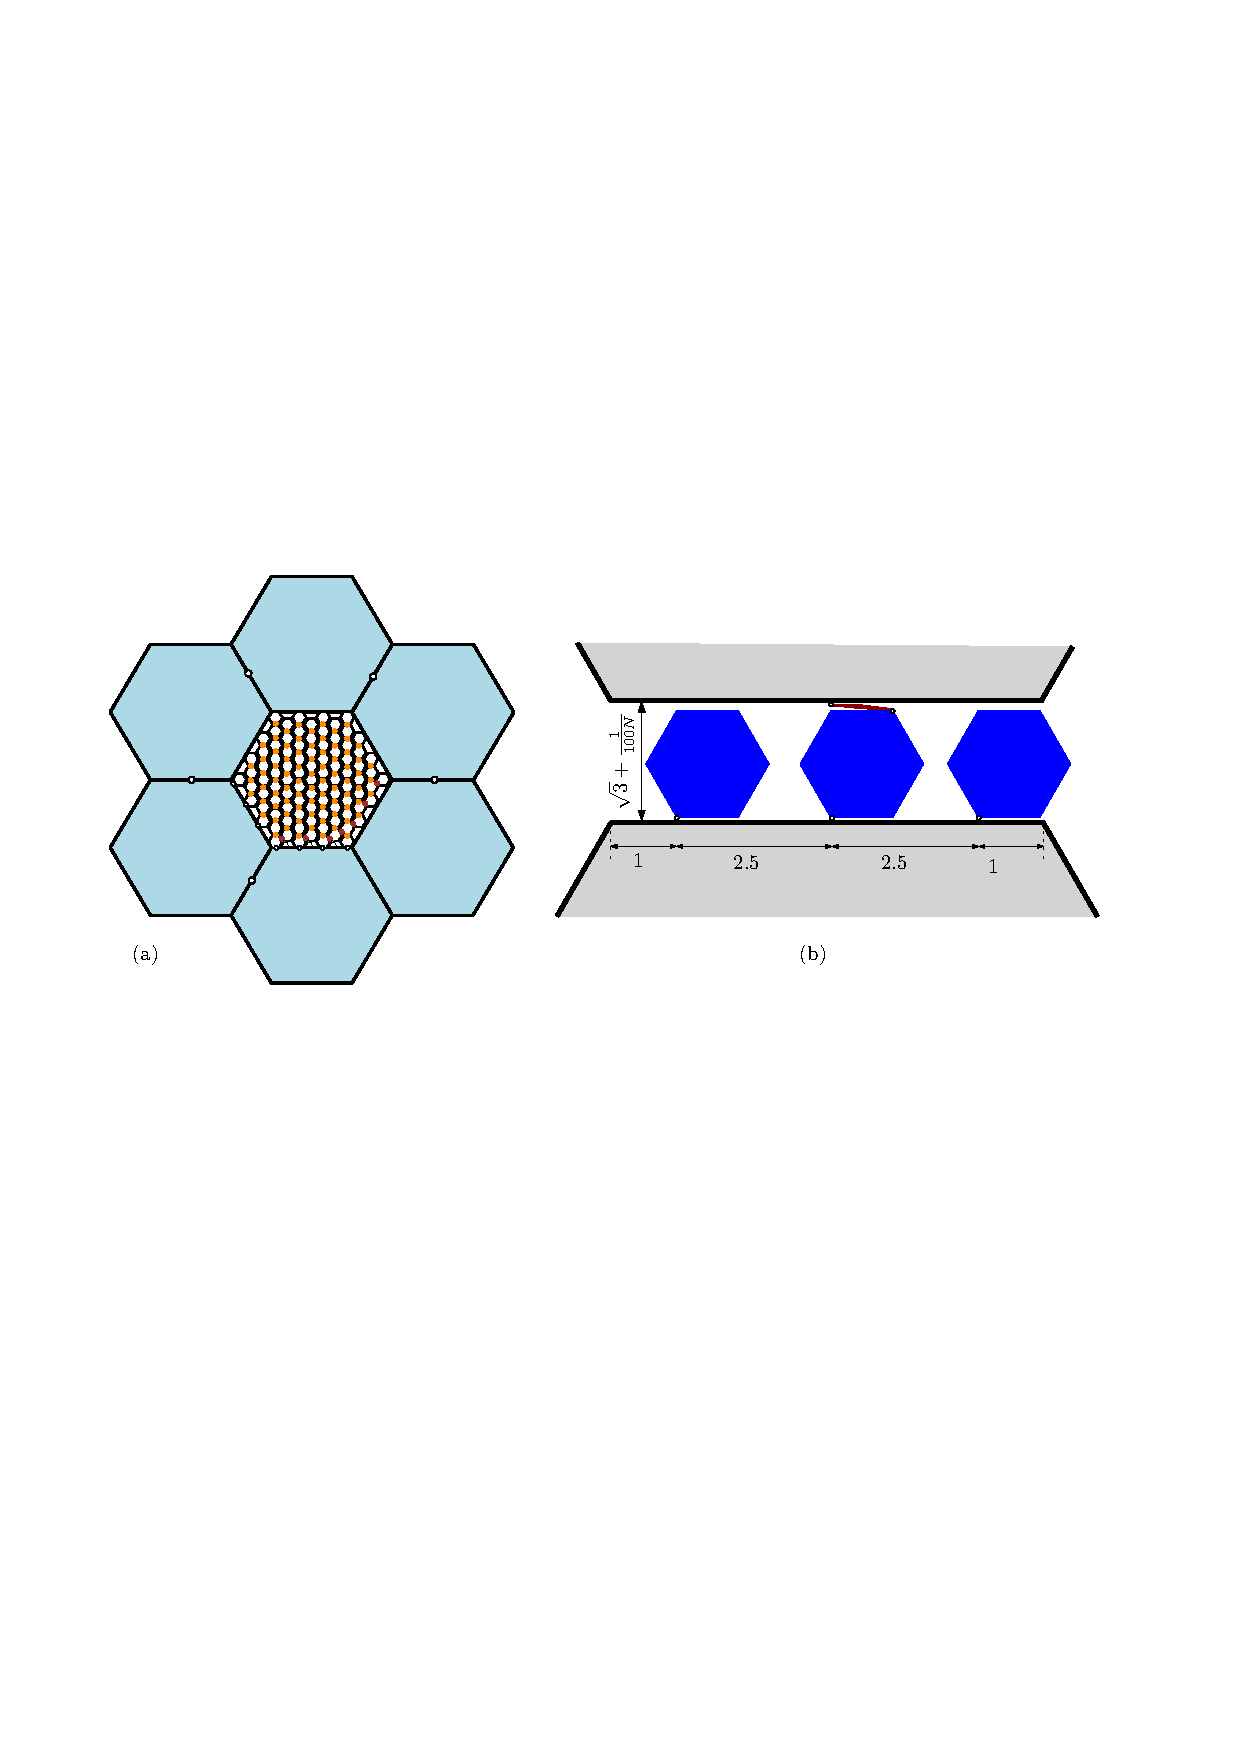
\includegraphics[width=0.95\columnwidth]{graphics/fig-frame-hex}
	\captionof{figure}{(a) A frame (built of 6 hinged regular hexagons) encloses a hexagonal tiling, and
    vertical paths connect all obstacle hexagons to the frame.
    (b) A corridor is widened to $\sqrt{3}+\frac{1}{N^2}$. A connection between
    two adjacent obstacle hexagons is established via a skinny rhombus.}
	\label{fig:frame}
	\end{center}
\end{minipage}

The position of each hexagon can be defined by the isometry from its canonical position; an isometry is given by the triple $\lr{\alpha, \beta, \delta}$ where $\alpha$ is a counter clockwise rotation about the center of the hexagon and $\lr{\beta,\delta}$ is a translation vector.  
Canonical position would have each obstacle hexagon's position as $(0,0,0)$.

\begin{lem}\label{lem:aux-C}
Let P be a polygonal linkage obtained from the modified auxilary construction.  
In every realization of $P$, the obstacle polygons are close to canonical position.
\end{lem}

Lemma \ref{lem:aux-C} serves as assurance that once a boolean formula of P3SAT is encoded into an arbitrary realization of the modified auxilary construction, the information of the boolean formula is preserved regardless of the positioning of the gadgets and components in the construction.
This quality shows that the information is stable and preserved in an arbitrary realization of the modified auxilary construction.
For example, in Figure \ref{fig:tiltedObstaclesInFrame.pdf}, we have a column of obstacle hexagons veering off $\ell$.

\begin{minipage}{\linewidth}
\begin{center}
\includegraphics[width=.3\columnwidth]{graphics/tiltedObstaclesInFrame.pdf}
\captionof{figure}{This figure depicts a column of obstacle hexagons rotated such that the obstacle hexagons veer of the vertical line $\ell$.}\label{fig:tiltedObstaclesInFrame.pdf}
\end{center}
\end{minipage}

This is an example of extreme angular rotation that should not occur over a vertical stack of hexagons. 
If a P3SAT boolean formula were encoded into such a realization, the information encoded could be lost by the extreme angular rotation of the obstacle hexagons.

\begin{proof}
We need to show that the modified auxilary construction could not deform in such a way that any information the construction encodes is lost or modified and the functionality of the gadgets within the construction behave as stated in the description.  
Using the central flag and rhombus, we can indentify a column of obstacle hexagons if there is a horizontal corridor between hexagons in canonical position.

\begin{minipage}{\linewidth}
\begin{center}
\includegraphics[width=.5\columnwidth]{graphics/dualSmallHexagonalGrid.pdf}
\captionof{figure}{(a) depicts a column of obstacle hexagons $O_1$, $\ldots$, $O_{10}$ along the vertical line $\ell$; (b) identifies obstacle hexgons $O_1$, $\ldots$, $O_{10}$ in (a).}\label{fig:dualSmallHexagonalGrid.pdf}
\end{center}
\end{minipage}

Without loss of generality, we can identify a column of obstacle hexagons $O_i$ along a vertical line $\ell$ (See Figure \ref{fig:dualSmallHexagonalGrid.pdf}).
In this proof, unless otherwise specified, we assume that the argument refers to a column that starts and ends with an obstacle hexagon.  
In total there will be $u+1$ number of obstacle hexagons and $u$ corridors in a column.
Note that:
$$\begin{array}{rcl}
u&=& \frac{J_h (z)}{2} - \frac{1}{2}\\
&=& \frac{1}{2}\lr{6z + 1 - 1}\\
&=& 3z\\
&=& 12s
\end{array}$$
where $J_h$ is defined in Equation \ref{eqn:Jh}.

The width of a skinny rhombus in canonical position is $\frac{1}{100N}$.
The obstacle hexagon has height of $ 2 N(n,m) \sqrt{3}$, and the flag is of height $\sqrt{3}$. 
The height $H(n,m)$ (and $\ell$ in Figure \ref{fig:corridorNonCanonical.pdf}(a)) can be expressed as a sum of the heights of the corridors and obstacle polygons:
$$(u+1) 2 N \sqrt{3} + u \lr{\sqrt{3}+ \frac{1}{100N}}$$
which reduces to:
\begin{eqnarray*}
(u+1) 2 N  \sqrt{3} + u \lr{\sqrt{3}+ \frac{1}{100N}}&=&(12s+1) 2 \frac{5t-1}{2}  \sqrt{3} + 12s \lr{\sqrt{3}+ \frac{1}{100\frac{5t-1}{2}}}\\
&=&(12s+1)  (5t-1)  \sqrt{3} + 12s \lr{\sqrt{3}+ \frac{1}{250s^\kappa-50}}
\end{eqnarray*}

\begin{equation}\label{eqn:Hnm}
	H(n,m) = (12s+1)  \lr{5s^\kappa -1}  \sqrt{3} + 12s \lr{\sqrt{3}+ \frac{1}{250s^\kappa -50}}				
\end{equation}
\paragraph{Angular Rotation $\alpha$.}
First we show that the angular rotation of the obstacle hexagons with respect to canonical position is small.  
We first look at the relative angular difference between two adjacent obstacle polygons
$$\left\vert \alpha_i - \alpha_{i+1} \right\vert.$$
Given an arbitrary instance of a modified auxilary construction, consider $O_i$, $O_{i+1}$, and the corridor between $O_i$ and $O_{i+1}$ (see Figure \ref{fig:corridorNonCanonical2.pdf} for illustration).  
For this argument, we assume that $O_i$ is horizontal and consider the relative position of other objects with respect to $O_{i}$.

\begin{minipage}{\linewidth}
\begin{center}
\includegraphics[width=.9\columnwidth]{graphics/corridorNonCanonical2.pdf}
\captionof{figure}{The obstacle hexagon here is in noncanonical position, and showing the side lengths adjacent to $\alpha_i$.}\label{fig:corridorNonCanonical2.pdf}
\end{center}
\end{minipage}

Figure \ref{fig:corridorNonCanonical2.pdf} $O_{i+1}$ is in a non-canonical position.  We describe the paramaters of the figure:
\begin{itemize}[leftmargin=.75in, rightmargin=.75in]
	\item[$\xi$:] the half length of the corridor,
	\item[$\omega_i$:] the angle between the rhombus and central flag, 
	\item[$\gamma_i$:] the angle formed between the horizontal plane that is $\sqrt{3}$ above $O_i$ and $O_{i+1}$ when rotated to the maximal possible extent before causing possible collision with other flags. 
	\item[$\zeta_i$:]  is the length from the hinge point of $O_{i+1}$ and the rhombus to the point that vertical to corner of $O_i$ that is to the right over the central flag on the horizontal plane that is $\sqrt{3}$ above $O_i$.
	\item[$\phi_i$:] is the angle formed between the central flag and $O_i$.
\end{itemize}

In Figure \ref{fig:dualSmallHexagonalGrid.pdf}(a) we see $\ell$ in the center of the column of obstacle hexagons.  
Our goal is to show that the column of hexagons cannot tilt in the manner shown in Figure \ref{fig:tiltedObstaclesInFrame.pdf} where the column veers greatly into the space occupied by other corridors and obstacle hexagons.
The cross section of an arbitrary corridor must have a height of at least $\sqrt{3}$ everywhere. 
%noncanonical corridor must be at least 
Otherwise, a flag would overlap with an obstacle hexagon; it would no longer remain a realization since the height of a flag is $\sqrt{3}$.
In Figure \ref{fig:corridorNonCanonical2.pdf}, we illustrate an obstacle hexagon, its upper corridor with the central flag rotated counterclockwise $\frac{\pi}{6}$ radians that has a hinge to the skinny rhombus in a vertical position.  
The skinny rhombus has length $\sqrt{1 + \lr{100N}^{-2}}$.
The rhombus is hinged at the midpoint of the upper side of the corridor.
The length from a corridor's midpoint to one end of the corridor is $\frac{5t-1}{4}$.
$\gamma_i$ is the angle between $\zeta_i$ and the horizontal axis at the height of the flag ($i = 1,2,\ldots, u$).
The bound of $\gamma_i$ is:
\begin{equation}\label{eqn:alphaBound}
\begin{array}{rcl}
\gamma_i & \leq & \tan^{-1} \lr{
								\frac{\lr{2 - \sqrt{3}} + \sqrt{1 + \lr{\frac{1}{100N}}^2}	}
									 {	\frac{5t -1}{4}	}
								}\\
& \leq & \frac{
				4 \lr{2 - \sqrt{3}} + 4\sqrt{1 + \lr{\frac{1}{100N}}^2}	}
			  {	
			  	5t -1	
			  }\\
& \leq & \frac{
				\frac{4}{3} + \sqrt{16 + 9}	}
			  {	
			  	5t -1	
			  } \\

& \leq & \frac{\frac{19}{3}}{5t -1} \\
& \leq & \frac{\frac{24}{3}}{4s^\kappa} \\
&\leq& \frac{2}{s^\kappa}
\end{array} 
\end{equation}
Inequality \ref{eqn:alphaBound} uses the first term Maclaurin series of $\tan^{-1}$ (for reference, see table of Maclaurin series equations at the beginning of this chapter) and holds for sufficiently large $s$ and $\kappa$.  
Thus the relative rotational difference between adjacent obstacle hexagons is:
\begin{equation}\label{eqn:angularBound}
\left\vert \alpha_i - \alpha_{i+1} \right\vert \leq\frac{2}{s^\kappa}
\end{equation}
The relative difference between $\alpha_i$ and $\alpha_{i+1}$ is small.
The bottom most obstacle hexagon is hinged to the frame (see Figure \ref{fig:HalfSizeHexagon.pdf} for illustration). 
This implies that $\alpha_1 = 0$ and
$$\vlr{\alpha_1 - \alpha_2}=\vlr{\alpha_2}\leq \frac{2}{s^\kappa}.$$
There are a total of $u$ obstacle hexagons in a column with possibly up to $u-1$ nonzero obstcle hexagons rotations.
We can derive 1) a bounded sum of rotational displacement over a column of obstacle hexagons:
\begin{equation}\label{eqn:angularSumBound}
\sum_{i=1}^{u-1} \vert \alpha_i - \alpha_{i+1} \vert \leq \frac{2(12s-1)}{s^\kappa} \leq \frac{24}{s^{\kappa-1}}
\end{equation}
and 2) derive the maximum rotational displacement at the $\ith$ obstacle hexagon:
\begin{eqnarray*}
\alpha_i &\leq& \frac{2}{s^\kappa} \sum_{j=1}^i j\\
		 &\leq& \frac{2}{s^\kappa}  \frac{i^2+i}{2}\\
		 &\leq& \frac{2}{s^\kappa}  i^2\\
		 &\leq& \frac{2u^2}{s^\kappa}\\
		 &\leq& \frac{288s^2}{s^{\kappa}}\\
		 &\leq& \frac{288}{s^{\kappa-2}} \\
\end{eqnarray*}
For any $i$, the bound for $\alpha_i$:
\begin{equation}\label{eqn:angularMaxBound}
\alpha_i \leq \frac{288}{s^{\kappa-2}}
\end{equation}

% The sum of total displacement in a given column is bounded by:
% $$ \vert \alpha_u \vert \leq \sum_{i=2}^{u-1} \vert \alpha_i - \alpha_{i+1} \vert \leq \frac{u-1}{2\lr{N^3 - 1}}= \frac{12s - 1}{2 \lr{ (c_N s)^3 - 1}}$$

\paragraph{Vertical Displacement $\delta$}

When an obstacle hexagon is rotated by $\alpha_i$, the height of the obstacle hexagon becomes $h \sec \alpha_i$ where $h$ is the canonical height of the obstacle hexagon (see Figure \ref{fig:hexagonNonCanonical.pdf} for reference).
Figure \ref{fig:hexagonNonCanonical.pdf} shows the geometry of a rotated obstacle hexagon.

\begin{minipage}{\linewidth}
\begin{center}
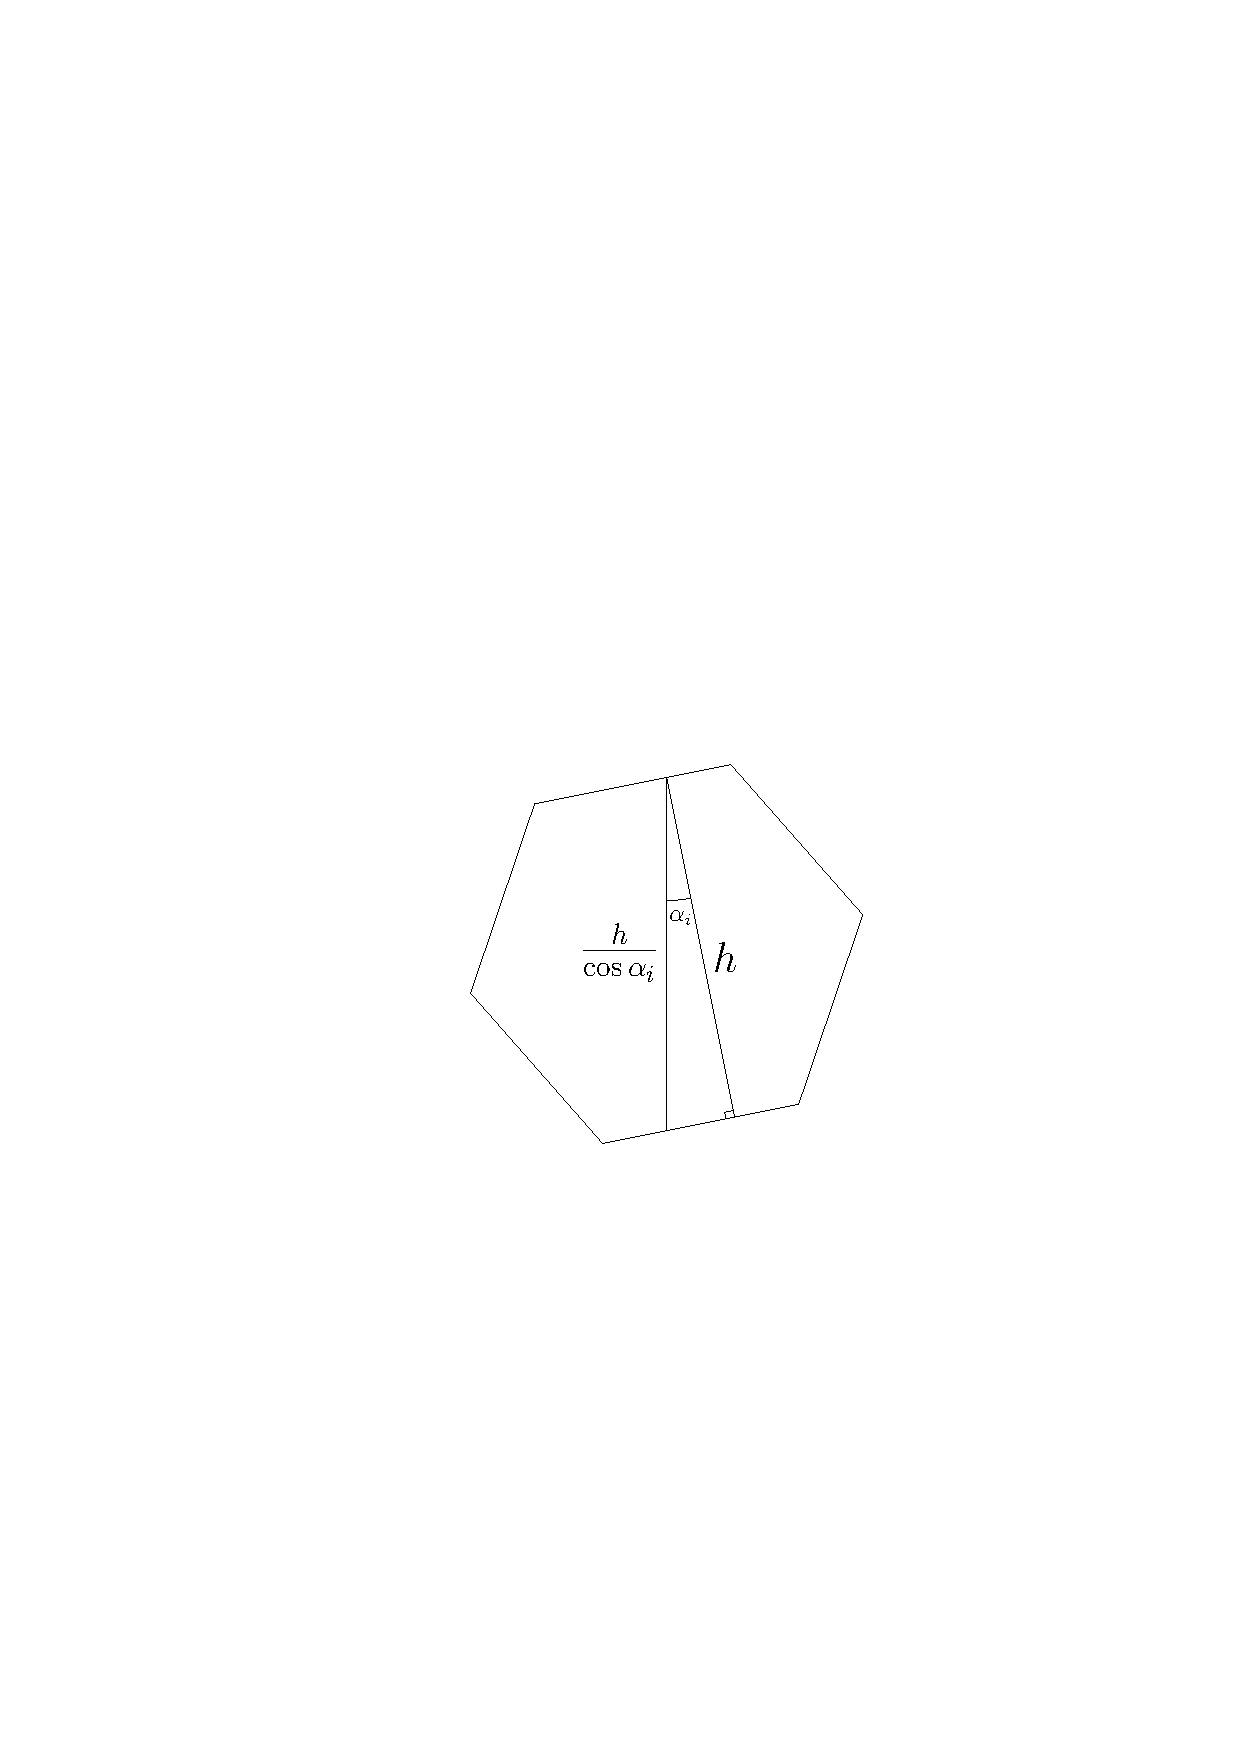
\includegraphics[width=.33\columnwidth]{graphics/hexagonNonCanonical2.pdf}
\captionof{figure}{
This figure shows a right triangle with angle $\alpha_i$ and sides of length $h$ and $\frac{h}{\cos \alpha_i}$.
}\label{fig:hexagonNonCanonical.pdf}
\end{center}
\end{minipage}

To show that the vertical displacement from canonical position is small, we first consider a column of obstacle hexagons in canonical position (see Figure \ref{fig:dualSmallHexagonalGrid.pdf} for illustration).  
For canonical position, the $\jth$ obstacle has $\delta_j = 0$.

\begin{minipage}{\linewidth}
\begin{center}
\includegraphics[width=.33\columnwidth]{graphics/verticalDisplacementArgument.pdf}
\captionof{figure}{This illustration is of a column of obstacle hexagons in canonical position along a vertical line segment $\ell$.}\label{fig:verticalDisplacementArgument.pdf}
\end{center}
\end{minipage}

From Equation \ref{eqn:Hnm}, we know the exact height of $\ell$ in terms of the heights of the corridors and obstacle hexagons in canonical position.  
Consider the first $j$ terms for the height of the column of obstacle hexagons and corridors for an arbitrary construction with angular rotation and vertical displacement for \textit{one} obstacle hexagon $\vert \delta_v \vert > 0$, where $j=2$, $\cdots$, $u+1$ and $1 < v \leq j$.
\begin{eqnarray*}
\sum_{i=1}^j \lr{2 \sqrt{3} N \sec \lr{ \alpha_i}} + \delta_v  + (j-1) \lr{\frac{1}{100N}+\sqrt{3}} &\leq& j \cdot 2 N \sqrt{3} + (j-1) \cdot \lr{\frac{1}{100N}+\sqrt{3}}\\
2 \sqrt{3} N \sum_{i=1}^j \sec \lr{\alpha_i} + \delta_ v &\leq& j \cdot 2 \sqrt{3} N \\
\sum_{i=1}^j \sec \lr{\alpha_i} + \delta_v &\leq& j\\
 \delta_v &\leq& j- \sum_{i=1}^j \sec \lr{\alpha_i}\\
 \delta_v &\leq& j - \lr{j - \sum_{i=1}^j \frac{\alpha_i^2}{2}}\\
\delta_v &\leq&  \sum_{i=1}^j \frac{\alpha_i^2}{2}
\end{eqnarray*}

Using Inequalities \ref{eqn:angularSumBound} and \ref{eqn:angularMaxBound}, we derive the following result:
$$
\begin{array}{rcl}
\sum_{i=1}^j \frac{\alpha_i^2}{2} &\leq& \frac{1}{2}\sum_{i=1}^j  \lr{ \frac{2}{s^\kappa} }^2\\
&\leq&\frac{1}{2}\cdot  \lr{\frac{2}{s^{\kappa}}}^2 \cdot j\\
&\leq&\frac{1}{2}\cdot  \lr{\frac{2}{s^{\kappa}}}^2 \cdot u\\
&\leq&\frac{48s}{2s^{2\kappa}}\\
&\leq&\frac{24}{s^{2\kappa-1}}\\  
\end{array}
$$

Thus we finally say that the bound for $\delta_v$, where $1<v\leq j\leq u$, is small:
\begin{equation}\label{eqn:verticalBound}
\delta_v \leq \frac{24}{s^{2\kappa-1}}
\end{equation}


\paragraph{\textit{A Refinement of the Angular Rotation Bound on $\alpha$}}
An obstacle hexagon can have at most a vertical displacement of $\delta_i$.  
A corridor's height can grow by $2 \delta_i$ should the obstacle below the corridor shift down by $-\delta_i$ and the obstacle above the corridor shift up $\delta_i$.  
We infer from our vertical bound Inequality \ref{eqn:verticalBound}:
$$\delta_i \leq \frac{12}{s^{2\kappa-1}}$$
By incorportating the new vertical bound, we extend the height of the corridor in Inequality \ref{eqn:alphaBound} to refine the bound on $\alpha$ as such:
\begin{equation}\label{eqn:alphaBoundRefined}
\begin{array}{rcl}
\gamma_i & \leq & \tan^{-1} \lr{
								\frac{\lr{2 - \sqrt{3}} + \sqrt{1 + \lr{\frac{1}{100N}}^2}	+ 2 \delta_i}
									 {	\frac{5t -1}{4}	}
								}\\
& \leq & \frac{
				4 \lr{2 - \sqrt{3}} + 4\sqrt{1 + \lr{\frac{1}{100N}}^2} + 8 \frac{24}{s^{2\kappa-1}}	}
			  {	
			  	5s^\kappa -1	
			  }\\
& \leq & \frac{
				\frac{4}{3} + \sqrt{16 + 9}	+  \frac{192}{s^{2\kappa-1}} }
			  {	
			  	5s^\kappa -1	
			  } \\

& \leq & \frac{\frac{19}{3}+\frac{192}{s^{2\kappa-1}}}{5 s^\kappa-1} \\
& \leq & \frac{200s^{2\kappa-1}}{4 s^\kappa \cdot s^{2\kappa-1}} \\
& \leq & \frac{50s^{2\kappa-1}}{ s^{3\kappa-1}} \\
&\leq& \frac{50}{s^{\kappa}}\\
\end{array} 
\end{equation}
\paragraph{Horizontal Displacement $\beta$}

There are two components of the modified auxiliary construction whose range of motion can create horizontal displacement, i.e. the skinny rhombi and the angular rotation of obstacle hexagons.  
Denote the horizontal displacement created by a skinny rhombi and rotational displacement as $\beta_\omega$ and $\beta_\alpha$ respectively.  
The skinny rhombi has a range of motion from the hinge of the center flag of the corridor.  
From canonical position, skinny rhombi can rotate clockwise about its hinge on the central flag.  
Without loss of generality, the $\ith$ skinny rhombus' non-canonical placement displaces the $\lr{i+1}^\text{st}$ obstacle hexagon.  
An obstacle hexagon's rotational displacement allows the hexagon to rotate about its hinge point with the skinny rhombus below it in an counter-clockwise manner about the skinny rhombus.  
Figure \ref{fig:someRangeSkinny.pdf} illustrates the two motions that generate $\beta_\omega$ and $\beta_\alpha$.

\begin{minipage}{\linewidth}
\begin{center}
\includegraphics[width=.9\columnwidth]{graphics/someRangeSkinny.pdf}
\captionof{figure}{(a) A pair of vertically adjacent obstacle hexagons and their corresponding corridor in canonical position.  (b) shows the same obstacle hexagons and corridors with the exception that the skinny rhombus is not in cannonical position. (c) is the same as (b) with the exception that the obstacle hexagon $O_{i+1}$ has rotation displacement.}\label{fig:someRangeSkinny.pdf}
\end{center}
\end{minipage}

The angle in the interior of the rhombus from the diameter of the rhombus to the bottom side of the rhombus is a constant $\hat{\omega}_i = \arctan \lr{\frac{1}{100N}}$.  
For non-canonical positions, let $\omega_i$ be the angular displacement between a copy of the diameter of the skinny rhombus in canonical position and the diameter of the skinny rhombus in non-canonnical position.
The range of $\omega_i$ is $\lr{0, \frac{4 \pi}{3} - 2 \hat{\omega}_i}$.
Figure \ref{fig:someRangeSkinny.pdf}(a) shows the cannonical position of all objects.  
Figure \ref{fig:someRangeSkinny.pdf}(b) illustrates some range of angular motion $\omega_i$ that a skinny rhombus can rotate on its hinge with a flag.  
Figure \ref{fig:someRangeSkinny.pdf}(c) shows a rotational displacement of $O_{i+1}$ with the skinny rhombus' angular displacement.

Formally, the horizontal displacement of obstacle hexagon $O_{i,j}$ is the sum $\beta_{i,j} = \beta_{\omega_{i-1,j}} + \beta_{\alpha_{i,j}}$.  
To show that for any $i$ and $j$ that $\beta_{i,j}$ is small, we will show that (1) $\beta_{\omega_{i-1,j}}$ is polynomial and small with Lemma \ref{lem:betaOmegaSmall} and (2) from Lemma \ref{lem:betaOmegaSmall} we will also show that it is infeasible for $\beta_{\alpha_{i,j}} > 0$.  

\begin{lem}\label{lem:betaOmegaSmall}
For any integers $i$ and $j$: 
$$\beta_{\omega_{i-1,j}} \leq \sqrt{C^2 - \delta_{\omega_{i-1}}}$$
where 
$$C^2 \leq 2 \lr{1 + \lr{\frac{1}{100N}}^2} \lr{1 - \cos\omega_{i-1}}$$
and
$$\delta_{\omega_{i-1}} \leq \frac{6s\lr{144s^2+12s}^2}{\lr{32s^{3\kappa}}}^2 $$
and 
$$
\omega_{i-1,j} \leq \frac{-2}{100 \lr{5 s^\kappa - 1}} + \frac{684530^3s^{5\kappa}}{ 5  s^{6 \kappa}} + \frac{684530s^{15\kappa}}{ 30  s^{18 \kappa}}
$$
\end{lem}

\begin{proof}

In \ref{fig:TheOmegaFigure.pdf}, the vertical and horizontal displacement formed by the angular rotation $\omega_i$ of the skinny rhombus is shown, $\delta_{\omega_i}$ and $\beta_{\omega_i}$ respectively. 

\begin{minipage}{\linewidth}
\begin{center}
\includegraphics[width=.37\columnwidth]{graphics/TheOmegaFigure.pdf}
\captionof{figure}{The vertical displacement $\delta_{\omega_i}$ and horizontal displacement $\beta_{\omega_i}$ created from the skinny rhombus rotation $\omega$.}\label{fig:TheOmegaFigure.pdf}
\end{center}
\end{minipage}

The maximal displacement of the $\ith$ vertical displacement is $\delta_i$; thus $\delta_{\omega_i} \leq \delta_i$.  
When considering the full range of motion of the skinny rhombus (ignoring the upper bound $\delta_i$ for the moment), the maximal length of vertical displacement by $\omega_i$ is when the diamater of the skinny rhombus is vertical:
$$\begin{array}{rcl}
\delta_{\omega_i} &=& \sqrt{1 + \lr{\frac{1}{100N}}^2 } - \frac{1}{100N}\\
&=& \sqrt{1 + \lr{\frac{1}{100 \lr{\frac{5t-1}{2}}}}^2} - \frac{1}{100 \lr{\frac{5t-1}{2}}}\\
&=& \sqrt{1 + \lr{\frac{1}{50 (5t-1)}}^2} - \frac{1}{50 (5t-1)}\\
&=& \sqrt{1 + \lr{\frac{1}{50 \lr{5s^\kappa-1}}}^2} - \frac{1}{50 \lr{5s^\kappa-1}}
\end{array}$$
For sufficiently large $s$ the upper bound of $\delta_i$ is smaller than the maximal length of $\delta_{\omega_i}$:
$$
\sqrt{1 + \lr{\frac{1}{50 \lr{5s^\kappa-1}}}^2} - \frac{1}{50 \lr{5s^\kappa-1}} \leq 
\frac{6s\lr{144s^2+12s}^2}{\lr{32s^{3\kappa}}^2}$$
Thus, we use the bound of $\delta_i$ in Inequality \ref{eqn:verticalBound} as the maximal value for $\delta_{\omega_i}$.  
To find the value of $\omega_i$ for when the height of $\delta_{\omega_i}$ equals $\frac{6s\lr{144s^2+12s}^2}{\lr{32s^{3\kappa}}^2}$, we solve for $\omega_i$ in the following formula:
$$\begin{array}{rcl}
\sin \lr{\hat{\omega}_i + \omega_i} &=& \frac{\frac{1}{100N} + \frac{6s\lr{144s^2+12s}^2}{\lr{32s^{3\kappa}}^2}}{\sqrt{1 + \lr{\frac{1}{100N}}^2 }}\\
\sin \lr{\arctan \lr{\frac{1}{50\lr{5s^\kappa - 1}}} + \omega_i} &=& \frac{\frac{1}{50 \lr{5s^\kappa-1}} + \frac{6s\lr{144s^2+12s}^2}{\lr{32s^{3\kappa}}^2}}{\sqrt{1 + \lr{\frac{1}{50 \lr{5s^\kappa-1}}}^2} }\\
\sin \lr{
			\arctan \lr{
							\frac{1}{50\lr{
											5s^\kappa - 1
										   }
								     }
					    }
	    } \cos \lr{\omega_i} + 
\cos \lr{
		\arctan \lr{
					\frac{1}{50\lr{
									5s^\kappa - 1
									}
							}
					}
		}  \sin \lr{\omega_i} &=& \frac{
											\frac{
													1024 s^{6\kappa} + 300 s\lr{144s^2+12s}^2  \lr{5s^\kappa-1}
													}{
													51200 s^{6\kappa} \lr{5s^\kappa-1}
													} 
				
										}{
										\sqrt{1 + \lr{\frac{1}{50 \lr{5s^\kappa-1}}}^2} 
										}
\end{array}$$
Using SAGE \cite{sage}, we compute $\omega_i$ as shown in Appendix A.  
The equation in appendix A can be simplified as such:
\begin{equation}\label{eqn:structure}
\begin{array}{lll}
\omega_i&=& \hat{\omega}_i \\
&+& \sum_{i=1}^7 \frac{c_i \cdot a_i}{800 d}
\end{array}
\end{equation}
where $a_1 = 400$, $a_2 = 200$, $a_3 = 25$, $a_4 = 16$, $a_5 = a_1$, $a_6 = a_2$, $a_7 = a_3$ and $c_i$ are shown Table \ref{table:ci}:

\begin{table}[h]
\begin{center}
\begin{tabular}{|R|L|}
\hline
c_1&-243s^4 \\\hline
c_2&-81s^3\\\hline
c_3&-27s^2\\\hline
c_4&5s^{5\kappa}\\\hline
c_5&1215s^{4+\kappa}\\\hline
c_6&405s^{3+\kappa}\\\hline
c_7&135s^{2+\kappa}\\\hline
\end{tabular}
\end{center}
\label{table:ci}
\caption{The $c_i$ values in Equation \ref{eqn:structure}.}
\end{table}

Equation \ref{eqn:structure} can be relaxed for sufficiently large $\kappa$ and $s$ as follows:
 \begin{equation}\label{eqn:relaxedStructure}
 \begin{array}{rcl}
 \omega_i &=& -\hat{\omega}_i + \arcsin \lr{ \frac{-97200s^4
-16200s^3
-675s^2+
80s^{5\kappa}+
486000s^{4+\kappa}+
81000s^{3+\kappa}+
3375s^{2+\kappa}}{800\left(5  s^{6  \kappa} - s^{5  \kappa}\right)
			\sqrt{
				\frac{62500 s^{2\kappa} - 25000 s^\kappa + 2501}{2500\lr{5s^\kappa - 1}^2}
			 }
 }
}\\
 &=& -\hat{\omega}_i + \arcsin \lr{ \frac{-97200s^4
-16200s^3
-675s^2+
80s^{5\kappa}+
486000s^{4+\kappa}+
81000s^{3+\kappa}+
3375s^{2+\kappa}}{800\left(5  s^{6  \kappa} - s^{5  \kappa}\right)
			\sqrt{
				\frac{62500 s^{2\kappa} - 25000 s^\kappa + 2501}{62500 s^{2\kappa}-25000 s^\kappa +2500}
			 }
 }
}\\
 &=& -\hat{\omega}_i + \arcsin \lr{ \frac{-97200s^4
-16200s^3
-675s^2+
80s^{5\kappa}+
486000s^{4+\kappa}+
81000s^{3+\kappa}+
3375s^{2+\kappa}}{800\left(5  s^{6  \kappa} - s^{5  \kappa}\right)
			\sqrt{
				1+ \frac{1}{2500 \lr{1-5s^\kappa}^2}
			 }
 }
}\\
 &\leq& -\hat{\omega}_i + \arcsin \lr{ \frac{-97200s^4
-16200s^3
-675s^2+
80s^{5\kappa}+
486000s^{4+\kappa}+
81000s^{3+\kappa}+
3375s^{2+\kappa}}{2\left(5  s^{6  \kappa} - s^{5  \kappa}\right)
			\sqrt{
				1+ \frac{1}{2500 \lr{1-5s^\kappa}^2}
			 }
 }
}\\
 &\leq& -\hat{\omega}_i + \arcsin \lr{ \frac{-97200s^4
-16200s^3
-675s^2+
80s^{5\kappa}+
486000s^{4+\kappa}+
81000s^{3+\kappa}+
3375s^{2+\kappa}}{\left(5  s^{6  \kappa} - s^{5  \kappa}\right)
			\sqrt{
				4+ \frac{4}{2500 \lr{1-5s^\kappa}^2}
			 }
 }
}\\
 &\leq& -\hat{\omega}_i + \arcsin \lr{ \frac{-97200s^4
-16200s^3
-675s^2+
80s^{5\kappa}+
486000s^{4+\kappa}+
81000s^{3+\kappa}+
3375s^{2+\kappa}}{3\lr{ 5  s^{6 \kappa} - s^{5 \kappa} } } 
}\\
 &\leq& -\hat{\omega}_i + \arcsin \lr{ \frac{
97200s^{5\kappa}
16200s^{5\kappa}
675s^{5\kappa}+
80s^{5\kappa}+
486000s^{5\kappa}+
81000s^{5\kappa}+
3375s^{5\kappa}}{ 5  s^{6 \kappa} } 
}\\
 &\leq& -\hat{\omega}_i + \arcsin \lr{ \frac{684530s^{5\kappa}}{ 5  s^{6 \kappa} } 
}\\
&\leq& -\frac{1}{100N} + \frac{684530s^{5\kappa}}{ 5  s^{6 \kappa} } + \frac{\lr{\frac{684530s^{5\kappa}}{5  s^{6 \kappa}}}^3}{6}\\
&\leq& \frac{-2}{100 \lr{5 s^\kappa - 1}} + \frac{684530^3s^{5\kappa}}{ 5  s^{6 \kappa}} + \frac{684530s^{15\kappa}}{ 30  s^{18 \kappa}}
\end{array}
\end{equation}

Using the law of cosines, we establish:
$$C^2 \leq 2 \lr{1 + \lr{\frac{1}{100N}}^2} \lr{1 - \cos\omega_{i-1}}.$$
Finally, we can conclude:
$$\beta_{\omega_{i-1,j}} \leq \sqrt{C^2 - \delta_{\omega_{i-1}}^2}$$
\end{proof}

In order to show that $\beta_{\alpha_{i,j}}$ to be greated than zero, $\omega_{i-1,j}$ must be greater than $\frac{pi}{2} - \hat{\omega}_i$.  
There are two cases when this this happens.  
The first case is when $$\delta_{\omega_{i-1,j}} = \sqrt{1 + lr{\frac{1}{100N}}^2} - \frac{1}{100N}$$.  
The second case is when we the following:
$$\left\lbrace\begin{array}{rcl}
\delta_{\omega_{i-1,j}} &=& \sqrt{1 + lr{\frac{1}{100N}}^2}\\
\beta_{\omega_{i-1,j}} &>& \sqrt{C^2 - \delta_{\omega_{i-1}}^2}
\end{array}\right\rbrace				
$$.  
Lemma \ref{lem:betaOmegaSmall} rules out case 2.  
The first case is ruled out if we show:
$$\frac{6s\lr{144s^2+12s}^2}{\lr{32s^{3\kappa}}^2} < \sqrt{1 + lr{\frac{1}{100N}}^2} - \frac{1}{100N}$$
(proof goes here) 
\textbf{Lemma \ref{lem:aux-C} Conclusion.} 
Reviewing the bounds in the proof of Lemma \ref{lem:aux-C}, the proof suffices by letting $\kappa = 1$.  
We have thus shown that the triple $(\alpha, \beta, \delta)$ for any obstacle hexagon is small and bounded.  
Therefore the entire modified auxiliary construction in any realization is canonical or close to canonical where the encoded P3SAT information is stable.
\end{proof}
\begin{lem}\label{lem:lePieceDuResistance}
Lemma 3. For every instance $\Phi$ of P3SAT, the corresponding modified auxiliary construction
has the following properties: (1) it has polynomial size; (2) the hinge graph of the modified auxilary con-
struction is a tree; (3) it admits a realization such that the obstacle polygons remain fixed if and only if $\Phi$ is
satisfiable.
\end{lem}
\begin{proof}
\noindent (1) We can bound the number of obstacle hexagons to represent a variable gadget by $2 D$, where $D = \lr{ \max_{v \in V} \deg (v)}$.  
The number of clause junctions is $n$.
To give an upper bound on the number of flexible hexagons in the auxiliary construction, we have to account for the flexible hexagons in the transmitter gadgets, the extra hexagons found in junctions, and the flexible hexagons around the variable gadgets.

Recall that that the number of flexible hexagons in a corridor are $ t = 2N(m,n)^3 + 1 $ where $N(m,n)$ is a polynomial. 
Recall that the drawing of $A(\Phi)$ have edges drawn in vertically and horizontally and can join at some ``elbow''.  
The distance can be measured in the $\ell_1$ norm.
Similarly in the honeycomb construction, the flexable hexagons zig-zig vertically and horizontally through out honeycomb.  
The number of corridors about an obstacle hexagon is $6$.
To give a generous upper bound on the number of flexible hexagons in a transmitter gadget, is $6 \cdot t \cdot \ell_1\lr{v_i,C_j}$, assuming each obstacle hexagon is of unit height.

The number of junctions in the auxiliary construction is the number of junctions to form all variable gadgets, transmitter gadgets, and clause gadgets. 
We know there are at most $2 \cdot D$ obstacle hexagons to form each variable gadget and $6$ junctions for each obstacle hexagon.  
Therefore an upper bound for the number of flexible hexagons around variable gadgets is $m \cdot 6 \cdot t \cdot 2 \cdot D$.
The upper bound for the number of junctions in a transmitter gadget is $6 \ell_1 \lr{v_i, C_j}$.  
Thus, the upper bound of all junctions in all transmitter gadgets is $$6 \cdot \sum_{\left\lbrace v_i, C_j \right\rbrace \in E} \ell_1 \lr{v_i, C_j}.$$
The upper bound on the total number of flexible hexagons is
$$m \cdot 6 \cdot t \cdot 2 \cdot D + 6 \cdot \sum_{\left\lbrace v_i, C_j \right\rbrace \in E} \ell_1 \lr{v_i, C_j}.$$

For each corridor, there is one skinny rhombus attached to one flexible hexagon in the corridor.  If the number of corridors is bounded polynomially, then the number of skinny rhombi is bounded by the same bound of the corridor.

\noindent (2) Recall that in the original auxilary construnction is a forest.
each obstacle hexagon with hinged flexible hexagons (and small hexagons) is disjoint from the remainder of the the construction. 
The skinny rhombi in the modified auxilary construction connect the disjointed trees to form one tree.

\noindent (3) The final statement is to show an if and only if statement: the modified auxiliary construction admits a realization such that the obstacle polygons remain fixed if and only if $\Phi$ is satisfiable.

Suppose $\Phi$ is satisfiable.  % and has $m$ variables $x_1$ through $x_m$ and $n$ clauses $C_1$ through $C_n$.
Each variable has a boolean value and we can encode a corresponding auxilary construction and then modify it as a modified auxiliary construction.
For each variable, we encode the boolean value by the state of the flags surrounding the variable gadget to $R$ or $L$.  
Lemma \ref{lem:aux-2} shows that the corridors and junctions around the variable gadget are realizable.
Lemma \ref{lem:aux-3} also show that for each transmitter gadget, every corridor and junction are also realizable. 
Lemma \ref{lem:aux-1} shows that there is at least one hexagon in the clause junction and that the clause is realizable.
Thus all parts of the auxilary construction realizable.  
Transforming it insto a modified auxilary construction and by Lemma \ref{lem:aux-C}, the modified auxiliary construction is realizable.

Suppose the construction admits a realization such that the obstacle polygons remain fixed.
Each variable gadget's flags are configured to state $L$ or $R$. 
The variable's corresponding state correspond to the variable's truth value, i.e. $R$ for true and $L$ for false.
Using Lemma \ref{lem:aux-2}, the boolean state of the variable gadget is transmitted to all transmitter gadgets associated to it.
Each clause is realizable and so for every clause, there exists one true literal in the clause corresponding to a variable by Lemma \ref{lem:aux-1}. 
If every clause has some true literal, then the corresponding 3-CNF boolean formula is satisfiable.
\end{proof}

At the beginning of this chapter, we stated Theorem \ref{thm:hinge2}: It is strongly NP-hard to decide whether a polygonal linkage whose hinge graph is a tree can be realized with counter-clockwise orientation.  
We know the P3SAT is NP-hard \cite{lichtenstein1982planar} and by Lemma \ref{lem:lePieceDuResistance}, we can conclude that deciding whether modified auxiliary construction (a tree) of a given P3SAT Boolean formula is NP-Hard.


% (0) It looks great in general. There are a few small corrections to make: in Figure 12(a), the bottom frame hexagons should have high degree (3 or 4), since each of them is incident to several columns of obstacle hexagons. The "half-size" hexagons shown in Figure 13 should also be represented in Figures 12(b) and Figure 14(a).
% (1) The degree of a variable vertex could be up to m, the number of clause vertices (e.g., when a variable appears in all clauses).
% Since the associated graph is bipartite and planar, Euler's formula implies that the sum of degrees of the variable vertices is at most 2m.
% (2) 
% Inequality (1.5) is correct. The coefficient 4 currently looks like a 4th root. Perhaps it would make sense to add a "\cdot" for multiplication. Also, when you use a Maclaurin series, the last negative term can be omitted for an upper bound. There some room for simplification. The sentence "it is clear that for N sufficiently large, gamma->0" is technically incorrect, it is true that if N goes to infinity, then gamma goes to 0; but we with to choose a polynomial size N. I would just delete that sentence, since it is clear anyways. In (1.6) and (1.7), the delta_i should be delta_j, right? That's why both of these inequalities give an upper bound for delta_j. Here sec(alpha) can be lower-bounded by 1; and the number of corridors should be (u-j) on both sides of the inequality.
% Also at the calculations above Figure 19 are no longer needed (they would bound the angle, not the vertical displacement).
% For bounding the horizontal displacement, draw a horizontal line across a "row" of obstacle hexagons. We can do this because the anle and the vertical displacement are already bounded. Then use the same argument as in (1.6) and (1.7), with a slightly adjusted argument. Specifically, we need to tell what the cross section of a corridor would be in the canonical position. It is (sqrt{3}+1/(100N)/sin(pi/6)  with our current parameters. If the two obstacles on the two sides of the corridor have some angle error alpha and vertical error delta, then the horizontal cross-section of the corridor may be smaller, but only a little bit smaller (use trig to approximate the cross-section).
% (3) Yes, s(n,m) and z(m,n) are related. A square grid of size sXs can be embedded in a honeycomb in a large hexagon of side length z=ceiling(sqrt{3}) s, or simply z=4s.